%% LyX 1.6.5 created this file.  For more info, see http://www.lyx.org/.
%% Do not edit unless you really know what you are doing.
\documentclass[12pt,a4paper,twoside,english,portrait]{article}
\usepackage[T1]{fontenc}
\usepackage[latin1]{inputenc}
\pagestyle{headings}
\usepackage{color}
\usepackage{babel}

\usepackage{graphicx}
\usepackage[unicode=true, 
 bookmarks=true,bookmarksnumbered=false,bookmarksopen=false,
 breaklinks=true,pdfborder={0 0 0},backref=false,colorlinks=true]
 {hyperref}
\hypersetup{pdftitle={CanReg5 - Instructions},
 pdfauthor={Morten Johannes ERVIK},
 pdfsubject={How to set up, run and work with CanReg5},
 pdfkeywords={CanReg5, Cancer registration}}
 
\makeatletter
%%%%%%%%%%%%%%%%%%%%%%%%%%%%%% Textclass specific LaTeX commands.
\newenvironment{lyxcode}
{\par\begin{list}{}{
\setlength{\rightmargin}{\leftmargin}
\setlength{\listparindent}{0pt}% needed for AMS classes
\raggedright
\setlength{\itemsep}{0pt}
\setlength{\parsep}{0pt}
\normalfont\ttfamily}%
 \item[]}
{\end{list}}

%%%%%%%%%%%%%%%%%%%%%%%%%%%%%% User specified LaTeX commands.
%% ================================================================================
%% This LaTeX file was created by AbiWord.                                         
%% AbiWord is a free, Open Source word processor.                                  
%% More information about AbiWord is available at http://www.abisource.com/        
%% ================================================================================
\usepackage{calc}\usepackage{fixltx2e}\usepackage{multicol}\usepackage[normalem]{ulem}%% Please revise the following command, if your babel
%% package does not support English (US)
\@ifundefined{definecolor}
 {\usepackage{color}}{}
\usepackage{hyperref}
%% \lfoot{\today}

\makeatother

\begin{document}
\begin{center}

\includegraphics[width=2.24931in,height=2.24931in]{0}
\par\end{center}

\begin{center}
\textbf{Open source} 
\par\end{center}

\begin{center}
By: Morten Johannes Ervik, IARC 
\par\end{center}

\begin{center}
Version: \today
\par\end{center}

\tableofcontents{}


\section{\textsf{Introduction}}

\begin{flushleft}
CanReg5 is an open source tool to input, store, check and analyse
cancer registry data. It has modules to do data entry, quality control,
consistency checks and basic analysis of the data. The main improvements
from the previous version are the new database engine, the improved
multi user capacities and that the development is managed like an
open source project. Also included is a tool to facilitate the set
up of a new or modification of an existing database by adding new
variables, tailoring the data entry forms etc. 
\par\end{flushleft}

\begin{flushleft}
Version 5 of CanReg is now ready for download.
\par\end{flushleft}


\subsection{\textsf{A short introduction to the database structure in CanReg5}}

\begin{flushleft}
New in CanReg5 is the three level table structure. Where CanReg4 stored
everything in one big table of tumours, CanReg5 splits this information
in three tables: Patient, Tumour and Source. For each patient, you
can store as many tumour records as you need, and for each tumour
you can store as many source records as you need. This allows us to
do more with our databases, for example related to completeness by
counting number of sources, but it poses come problem that might require
manual intervention during the conversion process of a system from
CanReg4 to CanReg5. 
\par\end{flushleft}

\begin{flushleft}
For example, some of you might store multiple sources in each tumour
record in CanReg4. This should be split into several source records
for this tumour record in CanReg5, but this is not an easy task to
automate since all registries that have opted for this have solved
it in a different way in CanReg4. 
\par\end{flushleft}

\begin{flushleft}
One way around this is to put all the fields related to the source
table in CanReg5 so that you are sure not to loose any data, and then
start from the date you start using CanReg5 to store multiple source
records per tumour. 
\par\end{flushleft}

\begin{flushleft}
The best way, but a more time consuming one, is to set up the source
table (by editing the system definition XML) to only contain the data
you want to store per source and then work on the exported file from
CanReg4 and import additional source information at a later stage.
(General import of data is not yet functioning adequately in CanReg5
- only import \& migration of old data.) 
\par\end{flushleft}

\begin{flushleft}
You can of course choose not to use the source table, as well - just
record the source information per tumour like you would in CanReg4.
This can be set up while migrating your system definition files. 
\par\end{flushleft}


\subsection{\textsf{Forum, Issue tracker, community site, twitter}}

\begin{flushleft}
We have created a project page at Project Kenai to help us keep track
of issues with CanReg5: \href{http://kenai.com/projects/canreg}{http://kenai.com/projects/canreg}.
This consists of one open forum, one closed user forum and an issue
tracker (standard BugZilla). To have access to the user forum and
the issue tracker you need to create an account at Project Kenai and
ask to be associated with the CanReg project. This is free of charge.
Using these tools allows you to see what error reports other CanReg
users have already filed and if solutions have already been proposed
and also discuss potential improvements for CanReg5. 
\par\end{flushleft}

\begin{flushleft}
You can of course still send us emails. 
\par\end{flushleft}

\begin{flushleft}
If you encounter any problems please provide a description of it along
with the specifications of your computer. (Operating System (Windows
XP, Vista, OSX, Linux?), memory, processor speed etc.) Also it would
be very useful if you can precise the \textbf{version} and the\textbf{
build code} of your CanReg5. This can be found on the bottom left
of the welcome screen and on the {}``About'' screen. (For example
Version: {}``4.99.0b586'') 
\par\end{flushleft}

\begin{flushleft}
Please be aware that some problems can be avoided by installing the
latest version of the Java Runtime Environment (Version 6) before
you start. (Available from \href{http://java.com/en/download/manual.jsp}{http://java.com/en/download/manual.jsp}.) 
\par\end{flushleft}

\begin{flushleft}
Videos documenting certain operations described below can be downloaded
from: \href{http://www.iacr.com.fr/CanReg5/videos.zip}{http://www.iacr.com.fr/CanReg5/videos.zip}
. 
\par\end{flushleft}

\begin{flushleft}
Last, but not, least: CanReg has its own stream on twitter. Please
follow: \href{http://twitter.com/canreg}{http://twitter.com/canreg}
for updates. 
\par\end{flushleft}


\subsection{\textsf{Getting hold of the latest version of CanReg}}

\begin{flushleft}
If you are running version 4.99.1 (or newer) of CanReg, you can launch
CanReg and click {}``Options...'', go to the {}``Advanced'' tab.
There you see your current version, i.e. 4.99.1. If you click {}``Check''
CanReg will look for an updated version. Afterwards you can click
{}``Download latest version'' to get the zip-file containing the
most recent version of CanReg5. 
\par\end{flushleft}

\begin{center}
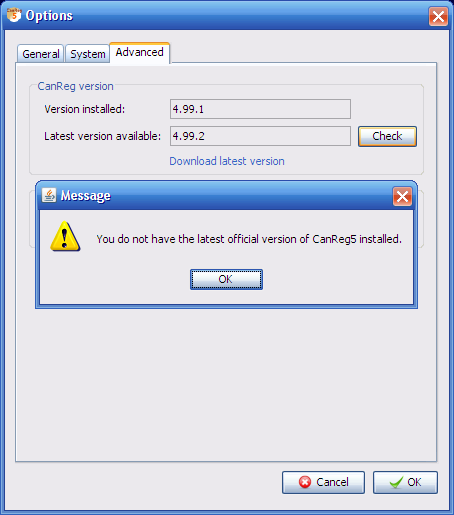
\includegraphics[width=4.72917in,height=5.36458in]{1}
\par\end{center}

\begin{flushleft}
If you have version 4.99.0 or no CanReg5 at all you can download the
newest version from here: \href{http://www.iacr.com.fr/CanReg5/CanReg5.zip}{http://www.iacr.com.fr/CanReg5/CanReg5.zip}
\par\end{flushleft}


\subsection{\textsf{Logfile}}

\begin{flushleft}
CanReg generates a logfile when you run it. This file is called canreg5client.log
and is located in your home folder (on windows it is most probably
under C:\textbackslash{}Documents and Settings\textbackslash{}<your
username> ) If you can attach this to emails with feedback/queries
it would be very useful. Please note that this file is overwritten
each time CanReg is started, so you need to {}``take it'' just after,
for example, your error occurs.%
\begin{minipage}[t]{1\columnwidth}%
Example log-file:
\begin{lyxcode}
<?xml~version=\textquotedbl{}1.0\textquotedbl{}~encoding=\textquotedbl{}windows-1252\textquotedbl{}~standalone=\textquotedbl{}no\textquotedbl{}?>

<!DOCTYPE~log~SYSTEM~\textquotedbl{}logger.dtd\textquotedbl{}>

<log>

<record>
\begin{lyxcode}
<date>2009-06-25T16:09:27</date>

<millis>1245938967921</millis>

<sequence>0</sequence>

<logger>canreg.client.CanRegClientApp</logger>

<level>INFO</level>

<class>canreg.client.CanRegClientApp</class>

<method>startup</method>

<thread>10</thread>

<message>CanReg~version:~4.99.9b668~(20090625160546)</message>
\end{lyxcode}
</record>

<record>
\begin{lyxcode}
<date>2009-06-25T16:09:31</date>

<millis>1245938971265</millis>

<sequence>1</sequence>

<logger>canreg.server.management.SystemDescription</logger>

<level>INFO</level>

<class>canreg.server.management.SystemDescription</class>

<method>debugOut</method>

<thread>11</thread>

<message>create~table~APP.PATIENT~(~PRID~INTEGER~NOT~NULL~PRIMARY~KEY~GENERATED~ALWAYS~AS~IDENTITY~(START~WITH~1,~INCREMENT~BY~1),~NEXT\_RECORD\_DB\_ID~INTEGER,~LAST\_RECORD\_DB\_ID~INTEGER,~\textquotedbl{}PERS\textquotedbl{}~VARCHAR(1)~,~\textquotedbl{}FAMN\textquotedbl{}~VARCHAR(15)~,~\textquotedbl{}FIRSTN\textquotedbl{}~VARCHAR(16)~,~\textquotedbl{}MAIDN\textquotedbl{}~VARCHAR(10)~,~\textquotedbl{}SEX\textquotedbl{}~VARCHAR(1)~,~\textquotedbl{}BIRTHD\textquotedbl{}~INTEGER,~\textquotedbl{}TRIB\textquotedbl{}~VARCHAR(2)~,~\textquotedbl{}ADDR\textquotedbl{}~VARCHAR(3)~,~\textquotedbl{}OCCU\textquotedbl{}~VARCHAR(2)~,~\textquotedbl{}DLC\textquotedbl{}~INTEGER,~\textquotedbl{}STAT\textquotedbl{}~VARCHAR(1)~,~\textquotedbl{}OBSOLETEFLAGPATIENTTABLE\textquotedbl{}~INTEGER,~\textquotedbl{}PATIENTID\textquotedbl{}~VARCHAR(8)~NOT~NULL~,~\textquotedbl{}PATIENTRECORDID\textquotedbl{}~VARCHAR(8)~NOT~NULL~UNIQUE~,~\textquotedbl{}PATIENTUPDATEDBY\textquotedbl{}~VARCHAR(16)~,~\textquotedbl{}PATIENTUPDATEDATE\textquotedbl{}~INTEGER,~\textquotedbl{}PATIENTRECORDSTATUS\textquotedbl{}~INTEGER,~\textquotedbl{}PATIENTCHECKSTATUS\textquotedbl{}~INTEGER)~</message>
\end{lyxcode}
</record>

...

</log>
\end{lyxcode}
%
\end{minipage}
\par\end{flushleft}


\section{Installing and running CanReg 5}


\subsection{\textsf{Install necessary helper applications}}

\begin{flushleft}
Before you install and run CanReg5 for the first time it is recommended
that you install the following helper applications. 
\par\end{flushleft}


\subsubsection{Java Runtime Environment }

\begin{flushleft}
Install the latest Java Runtime environment (May 2010: Version 6 Update
20 ) You can get that from here:\href{http://java.com/en/download/manual.jsp}{http://java.com/en/download/manual.jsp}
\par\end{flushleft}


\subsubsection{PostScript Viewer }

\begin{flushleft}
To view the tables generated by CanReg5 are PostScipt files. PostScript
is an open standard, so you can use many different tools to view them.
(You can in many cases even send them directly to a printer.) Mac
OS X and most Linux-distributions come with tools to view them by
default. 
\par\end{flushleft}

\begin{flushleft}
On Windows, the tool I recommend is the open sourced and free GSview. 
\par\end{flushleft}

\begin{flushleft}
To run GS View you need to install Ghostscript first. This can be
for example be downloaded from here: \href{http://pages.cs.wisc.edu/~ghost/doc/GPL/gpl864.htm}{http://pages.cs.wisc.edu/$\sim$ghost/doc/GPL/gpl864.htm}
(Scroll all the way down, under the heading Microsoft windows and
download the {}``GPL Ghostscript 8.64 for 32-bit Windows (the common
variety)'' (\href{http://mirror.cs.wisc.edu/pub/mirrors/ghost/GPL/gs864/gs864w32.exe}{http://mirror.cs.wisc.edu/pub/mirrors/ghost/GPL/gs864/gs864w32.exe}) 
\par\end{flushleft}

\begin{flushleft}
Run this file to install Ghostscript.
\par\end{flushleft}

\begin{flushleft}
Then you can get GS View from here: \href{http://pages.cs.wisc.edu/~ghost/gsview/get49.htm}{http://pages.cs.wisc.edu/$\sim$ghost/gsview/get49.htm}
(Most probably, you should pick the Win32 self extracting archive
- the first download option. \href{http://mirror.cs.wisc.edu/pub/mirrors/ghost/ghostgum/gsv49w32.exe}{http://mirror.cs.wisc.edu/pub/mirrors/ghost/ghostgum/gsv49w32.exe}) 
\par\end{flushleft}

\begin{flushleft}
Run this file to install GS View. 
\par\end{flushleft}


\subsection{\textsf{Install CanReg5}}

\begin{flushleft}
CanReg5 is distributed as a zip-archive. To install it simply extract
the content to a new folder, for example on your desktop. (It is important
to keep the same directory structure as inside the zip-file.) 
\par\end{flushleft}


\subsection{\textsf{Un-install CanReg5}}

\begin{flushleft}
If you wish to un-install CanReg5, delete the following folders (or
rename if you have anything valuable in them):\\
\textbackslash{}\textbackslash{}Documents and Settings\textbackslash{}<your
username>\textbackslash{}.CanRegClient\\
\textbackslash{}\textbackslash{}Documents and Settings\textbackslash{}<your
username>\textbackslash{}.CanRegServer
\par\end{flushleft}


\subsection{\textsf{Run CanReg5}}

\begin{flushleft}
Go to the folder you installed CanReg5 in and double click on the
coffee cup icon (CanReg.jar). (\textbf{If, at this point, CanReg5
does not start you might have to update your Java Runtime Environment
and retry}. (See above.) 
\par\end{flushleft}

\begin{flushleft}
CanReg 5 Welcome window:
\par\end{flushleft}

\begin{center}
\includegraphics[scale=0.5]{\string"C:/Documents and Settings/ervikm/My Documents/NetBeansProjects/CanReg/doc/CanReg5-Instructions/CanRegWelcomeScreen\string".eps}
\par\end{center}


\subsection{\textsf{Demo system}}

\begin{flushleft}
Included is the dictionary for the training system located in the
demo-folder in the zip-file. With this you can get a demo-system up
and running to test some data entry. To run this demo system, install
the TRN-file to set up the system. Afterwards you should import the
dictionary using {}``Data Entry'' - ''Edit dictionary'' and {}``Import
complete dictionary from a file'', before you start to enter data. 
\par\end{flushleft}


\subsection{\textsf{Install a new CanReg5 system}}

\begin{flushleft}
If you want to install an already provided system definition (for
example the demo system TRN) please click {}``Install New System''.
CanReg5 will present you with the following message:
\par\end{flushleft}

\begin{center}
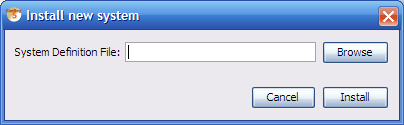
\includegraphics[width=4.20833in,height=1.30208in]{3}
\par\end{center}

\begin{flushleft}
Click browse to find the system definition file. (If you want to use
the TRN demo system look in demo/database and select TRN.xml and click
open and then Install.) 
\par\end{flushleft}


\subsection{\textsf{Convert the CanReg4 system definitions}}

\begin{flushleft}
If you have a CanReg4 system you can use tools built into CanReg to
help you migrate this to CanReg5. 
\par\end{flushleft}

\begin{flushleft}
First import the variables of CanReg 4 to CanReg 5 - the system definition
of CanReg4. 
\par\end{flushleft}

\begin{flushleft}
Go to {}``Tool'' in CanReg5 menu and click {}``Convert system definition''
\par\end{flushleft}

\begin{center}
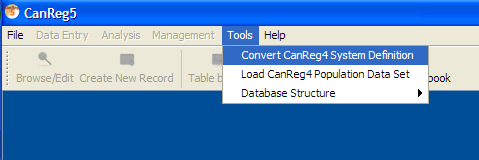
\includegraphics[width=4.17708in,height=1.42708in]{4}
\par\end{center}

\begin{flushleft}
Do {}``Browse'' to find your CanReg 4 system definition file. (This
is a file located in the folder \textbackslash{}\textbackslash{}CR4SHARE\textbackslash{}CANREG4\textbackslash{}CR4-SYST\textbackslash{}
followed by your 3 letter registry code i.e. TRN whose name is ending
in .DEF (i.e. CR4-TRN.DEF).) 
\par\end{flushleft}

\begin{flushleft}
Select your CanReg4 file and double click it or click {}``Open''. 
\par\end{flushleft}

\begin{flushleft}
Click {}``Convert''. 
\par\end{flushleft}

\begin{flushleft}
The program will then ask you if you want to add this server to your
favourites. Click {}``Yes'' here.
\par\end{flushleft}

\begin{center}
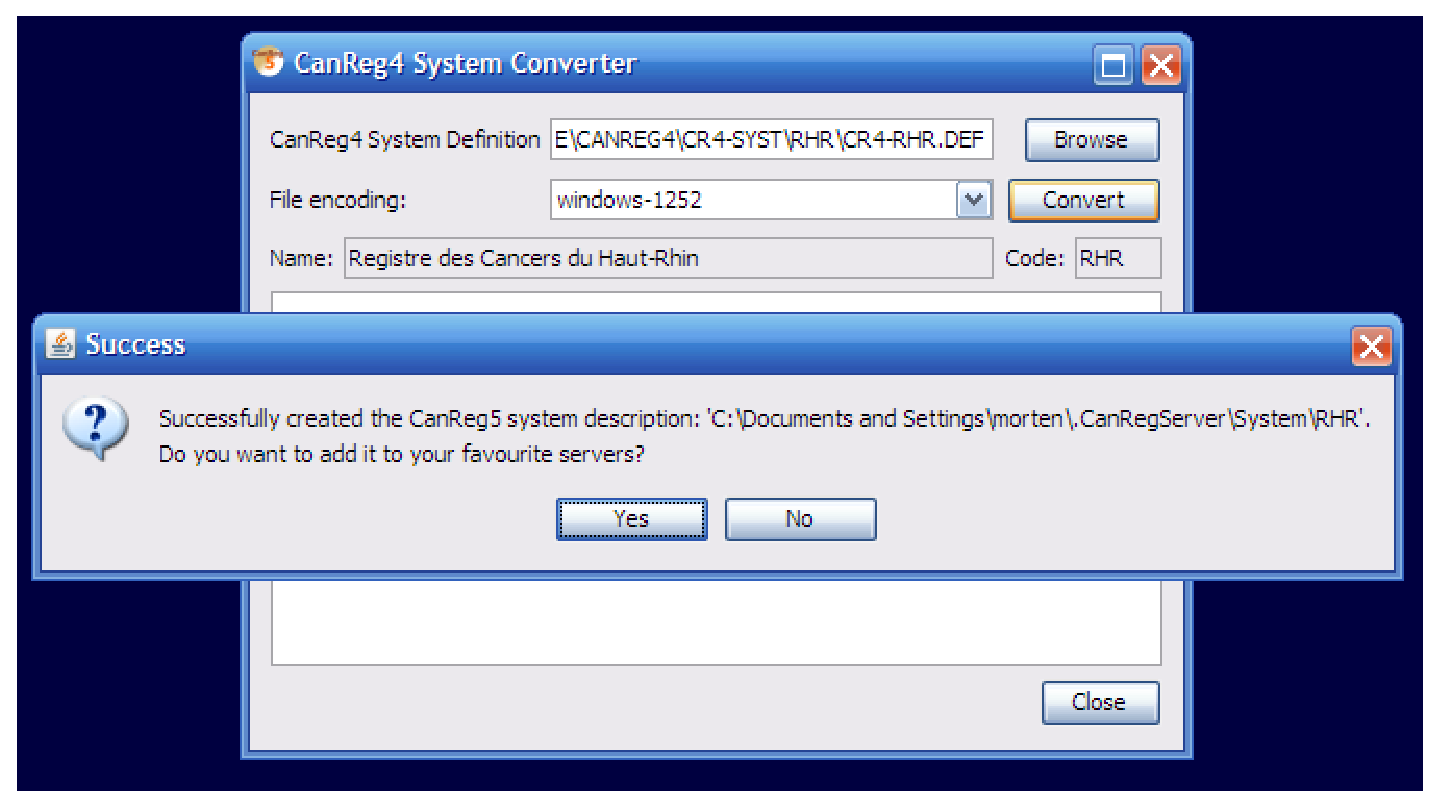
\includegraphics[width=5.4785in,height=3.1764in]{5}
\par\end{center}

\begin{flushleft}
The next step is the trickiest one during the conversion. Since we
go from a tumour based database structure with only one big table
with all the tumour and patient related information to a structure
with both a table for tumour related information and patient related
information we need to specify what variable goes in what table of
CanReg5. We recommend putting the unique patient related information
(name, date of birth and follow-up variables) in the patient table,
source information in the Source table and pretty much the rest (tumour
information, age, address etc) in the tumour table.
\par\end{flushleft}

\begin{center}
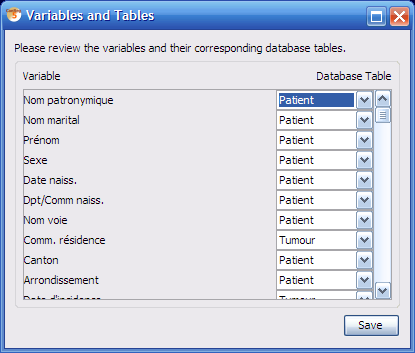
\includegraphics[width=4.32292in,height=3.67708in]{6}
\par\end{center}

\begin{flushleft}
The program presents an initial proposal that you might agree with,
but please go through one by one the variables and decide. 
\par\end{flushleft}

\begin{flushleft}
Click {}``Save''. You have now created an XML file that describes
your CanReg5 system. 
\par\end{flushleft}

\begin{flushleft}
{\footnotesize Optional: Before you proceed to the next step and launch
the server you can, if you want(!), manually edit this XML file you
have created by opening it in a text editor or a dedicated XML editor.
The file is located in your user folder under .CanRegServer. (On my
machine, for example, running Windows XP it is under: C:\textbackslash{}Documents
and Settings\textbackslash{}morten\textbackslash{}.CanRegServer\textbackslash{}System.)} 
\par\end{flushleft}


\subsection{\textsf{Setting up or modifying a CanReg system using the built in
editor}}

\begin{flushleft}
To modify an existing CanReg system or set up a new one you can use
tools built into CanReg5. 
\par\end{flushleft}

\begin{center}
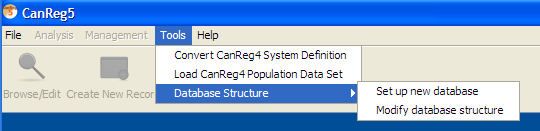
\includegraphics[width=5.4785in,height=1.3639in]{7}
\par\end{center}

\begin{flushleft}
They can be found under Tools -$>$ Database Structure. 
\par\end{flushleft}

\begin{center}
\textbf{Note: Before using this tool it is highly recommended to perform
a backup of your CanReg5 database!} 
\par\end{center}

\begin{flushleft}
For now please use {}``Set up new database''. This will give you
the Modify Database Structure window. 
\par\end{flushleft}

\begin{center}
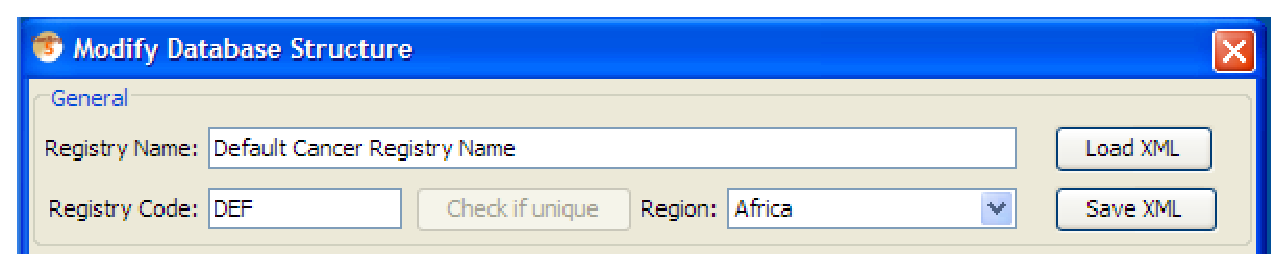
\includegraphics[width=5.4785in,height=1.0903in]{8}
\par\end{center}

\begin{flushleft}
Please click Load XML and either pick your own XML or, if you start
from scratch, the TRN.xml or DEF.xml found in the CanReg installation.
(You will need to load an existing XML to be able to create a working
XML for your CanReg system.) 
\par\end{flushleft}

\begin{flushleft}
Please note that certain modifications done using this tool will impact
the structure of the CanReg database to such an extent that it will
have to be rebuilt afterwards. Others like renaming groups, changing
the displayed name of a variable or reordering the variables are purely
cosmetic and do not impact the database structure as such. If you
wish to do changes to the structure of the database you'll need to
export your data prior to those changes, delete the database files
of the CanReg system, do required modifications using this tool or
directly in the XML, relaunching the CanReg server and then import
the data (this again will potentially have to be adapted to the structural
changes). 
\par\end{flushleft}

\begin{flushleft}
When this has loaded you'll see all the info specifying this CanReg
system. On the top you can specify the registry name, registry code
and region of the registry. Below you have a list of the Dictionaries,
then the Groups and then the Variables. 
\par\end{flushleft}

\begin{center}
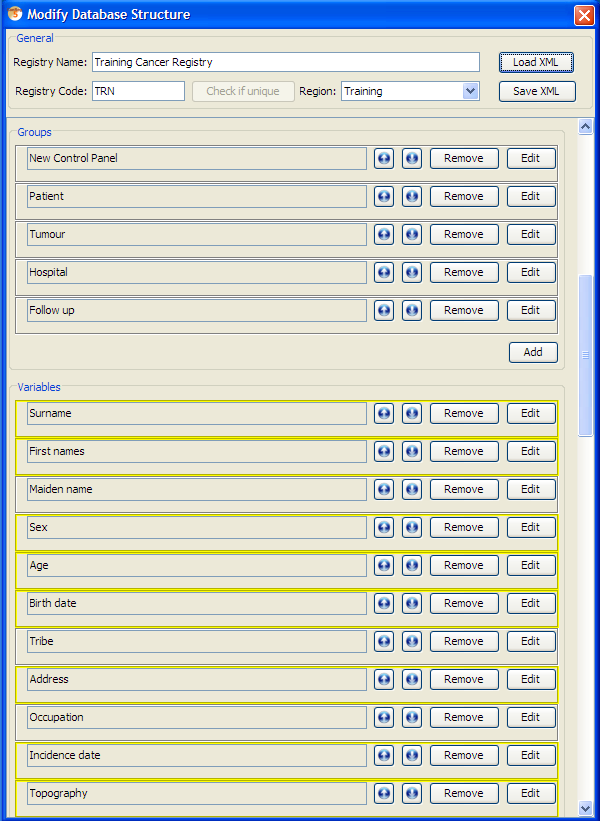
\includegraphics[width=5.4785in,height=7.884in]{9}
\par\end{center}

\begin{flushleft}
To add a dictionary, group or variable, click add in the proper pane.
This will then appear as the last item in the corresponding list for
you to edit. 
\par\end{flushleft}

\begin{flushleft}
Clicking edit on any button related to a dictionary, group or variable
brings up the respective editor. 
\par\end{flushleft}


\subsubsection{Modifying a dictionary }

\begin{center}
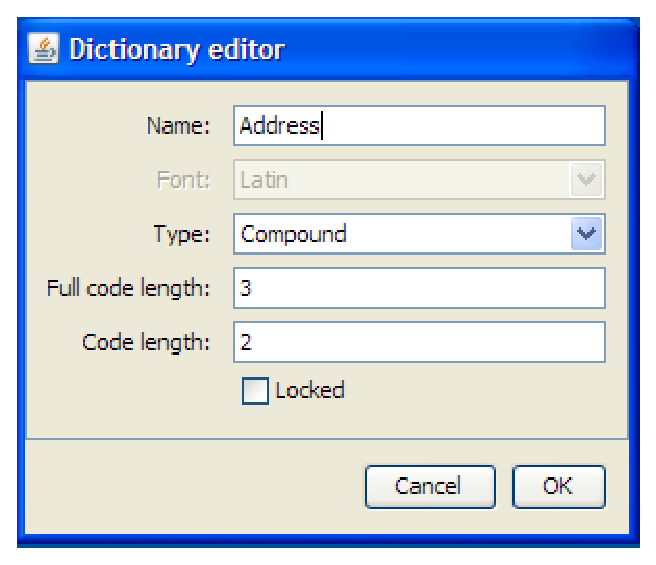
\includegraphics[width=3.11458in,height=2.65625in]{10}
\par\end{center}

\begin{flushleft}
Using the dictionary editor you can modify any dictionary in CanReg5.
The fields are as follows: 
\par\end{flushleft}

\begin{flushleft}
\textbf{Name:} The name of the dictionary 
\par\end{flushleft}

\begin{flushleft}
\textbf{Type:} This can either be {}``Simple'' or {}``Compound''.
A {}``Simple'' dictionary is a plain list of codes and corresponding
labels, whereas a {}``compound'' dictionary as two levels of refinement.
For example the user can pick the two first digits and then the last
digit, as in the above example. 
\par\end{flushleft}

\begin{flushleft}
\textbf{Full code length:} The number of character the codes for this
dictionary takes up in the database. 
\par\end{flushleft}

\begin{flushleft}
\textbf{Code length:} The number of characters in the first level
of refinement in the case of a compound dictionary. 
\par\end{flushleft}

\begin{flushleft}
\textbf{Locked:} Will you allow the super user to modify this dictionary
using the tools in CanReg, or should it be locked? 
\par\end{flushleft}


\subsubsection{Modifying a group }

\begin{center}
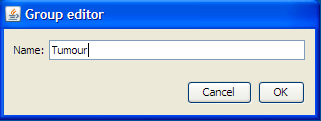
\includegraphics[width=3.34375in,height=1.26042in]{11}
\par\end{center}

\begin{flushleft}
Using the group editor you can modify any group in CanReg5. 
\par\end{flushleft}

\begin{flushleft}
\textbf{Name:} The name of the group 
\par\end{flushleft}


\subsubsection{Modifying a variable }

\begin{center}
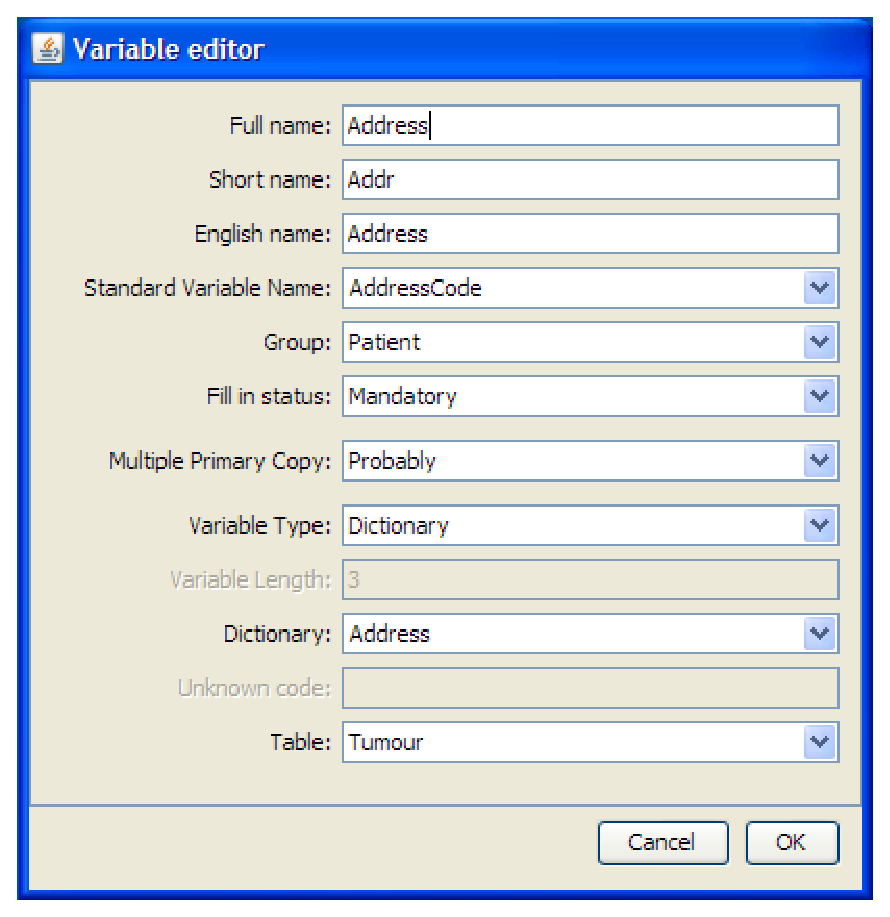
\includegraphics[width=4.28125in,height=4.41667in]{12}
\par\end{center}

\begin{flushleft}
Using the dictionary editor you can modify any variable stored in
the CanReg5 database. The fields are as follows: 
\par\end{flushleft}

\begin{flushleft}
\textbf{Full name:} The name of the variable as displayed in data
entry forms etc. 
\par\end{flushleft}

\begin{flushleft}
\textbf{Short name:} The name of the variable in the database. (This
should be without any blanks and other special characters and reasonably
short.) 
\par\end{flushleft}

\begin{flushleft}
\textbf{English name:} It is useful to provide an English name for
the variable in case you want to collaborate with people in other
countries. 
\par\end{flushleft}

\begin{flushleft}
\textbf{Standard Variable Name:} This maps the variable to a standard
CanReg5 variable for the purpose of edit checks and analysis. 
\par\end{flushleft}

\begin{flushleft}
\textbf{Group:} The choice of group only affects the display during
data entry. 
\par\end{flushleft}

\begin{flushleft}
\textbf{Fill in status:} Can be set to {}``Mandatory'', {}``Optional'',
{}``Automatic'' or {}``System'', depending on if you want to force
the registrar to provide this information before confirming the record. 
\par\end{flushleft}

\begin{flushleft}
\textbf{Multiple Primary Copy:} Legacy information. Leave as other. 
\par\end{flushleft}

\begin{flushleft}
\textbf{Variable Type:} Can be {}``Alphabetic'' (for plain text),
{}``Asian text'' (legacy field, same as {}``Alphabetic''), {}``Date'',
{}``Dictionary'', {}``Number'' and {}``Text Area''. 
\par\end{flushleft}

\begin{flushleft}
\textbf{Variable Length:} The length of the variable in characters. 
\par\end{flushleft}

\begin{flushleft}
\textbf{Dictionary:} If you chose {}``Dictionary'' as type of variable
you'll have to choose a dictionary here. 
\par\end{flushleft}

\begin{flushleft}
\textbf{Unknown code:} Here you can specify the unknown code of this
variable. 
\par\end{flushleft}

\begin{flushleft}
\textbf{Table:} Choose the table where this variable should be stored. 
\par\end{flushleft}


\subsubsection{Set up search variables }

\begin{center}
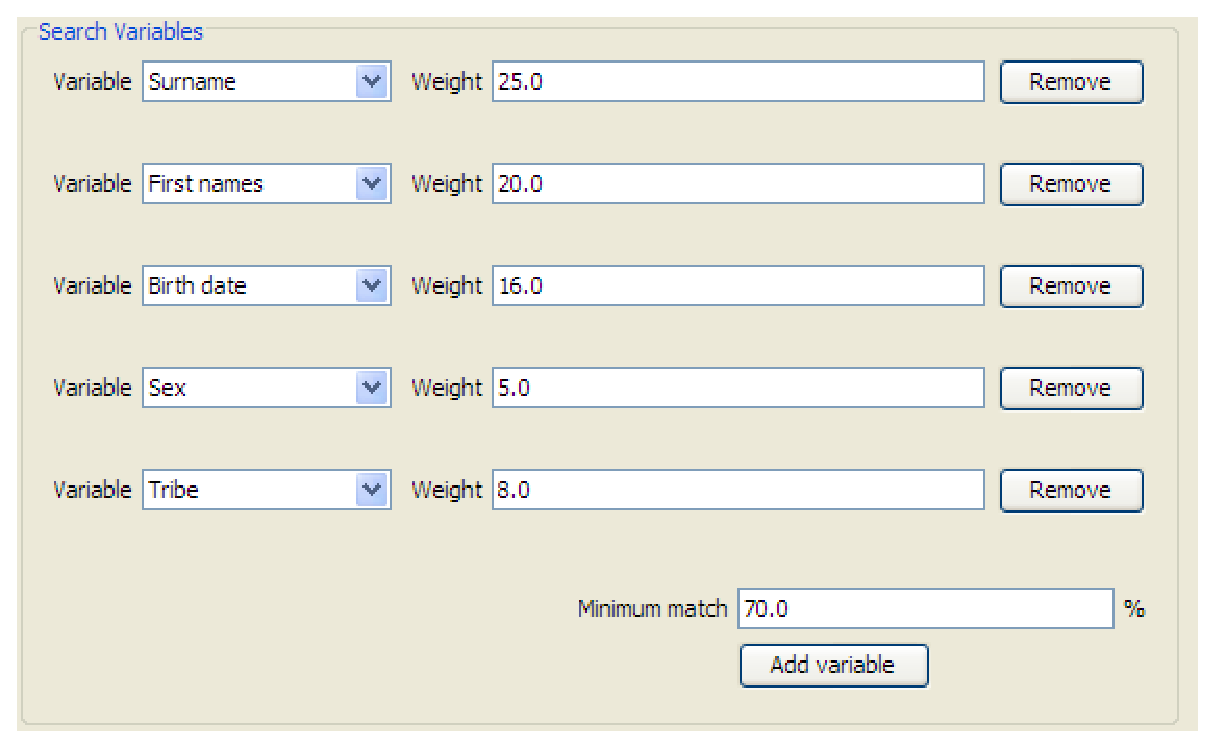
\includegraphics[width=5.4785in,height=3.4868in]{13}
\par\end{center}

\begin{flushleft}
Using this editor you can change the variables that come into play
during person search in CanReg5, and their respective weights and
minimum match criteria. 
\par\end{flushleft}


\subsubsection{Coding }

\begin{center}
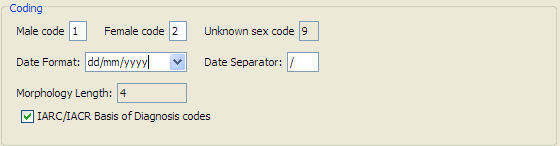
\includegraphics[width=5.4785in,height=1.5014in]{14}
\par\end{center}

\begin{flushleft}
Here you can change some coding settings of your CanReg system. (Not
yet implemented.) 
\par\end{flushleft}


\subsubsection{Settings }

\begin{center}
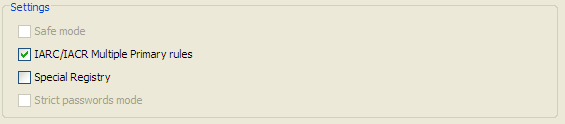
\includegraphics[width=5.4785in,height=1.2653in]{15}
\par\end{center}

\begin{flushleft}
Here you can change some settings of your CanReg system. (Not yet
implemented.) 
\par\end{flushleft}


\subsubsection{Saving the system }

\begin{flushleft}
By clicking Save XML the system XML will be saved to the system folder
of CanReg under the name $<$your system code$>$.xml (for example
TRN.xml), ready for use. 
\par\end{flushleft}


\subsection{\textsf{Launching the CanReg server}}

\begin{flushleft}
After clicking {}``Login'' on the welcome screen of CanReg you get
the login screen. To launch the CanReg server click {}``Settings''.
Click {}``Launch Server''. 
\par\end{flushleft}

\begin{center}
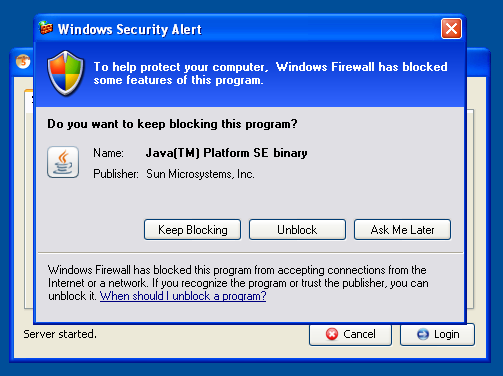
\includegraphics[width=5.23958in,height=3.91667in]{16} 
\par\end{center}

\begin{flushleft}
If you get a java firewall query, please confirm that it is OK that
java can comunicate through you firewall by clicking {}``Unblock'',
{}``OK'' or {}``Yes''. If this is the first time you launch the
server on this machine it will automatically create the database needed
for CanReg5. 
\par\end{flushleft}


\subsection{\textsf{Login}}

\begin{flushleft}
After launching the server you can log on to your CanReg system. 
\par\end{flushleft}


\subsubsection{Locally }

\begin{flushleft}
If you want to log in to a CanReg server running on your local machine,
after either installing a CanReg5 system XML or converted your CanReg4
system definition files you go to the {}``System'' tab of the {}``Login''-window
and choose your server from the drop down list. (Most probably already
selected.) (The default username is {}``morten'' and password is
{}``ervik''. (All in small letters with no double quotes.) Click
{}``Login'' and you'll be logged on.) 
\par\end{flushleft}

\begin{flushleft}
If you get an error message saying {}``Could not log in to the CanReg
server on localhost with the given credentials.'', please make sure
that you have entered the correct username and password and that the
server is indeed running. (See {}``Launching the CanReg server''
above.) 
\par\end{flushleft}

\begin{center}
\includegraphics{\string"C:/Documents and Settings/ervikm/My Documents/NetBeansProjects/CanReg/doc/CanReg5-Instructions/CanRegLoginScreen\string".eps}
\par\end{center}


\subsubsection{In a network }

\begin{flushleft}
If you want to log on to a CanReg server running on another machine
in your network you need to know the address of that machine. (Either
it's IP address or name on the network.) 
\par\end{flushleft}

\begin{flushleft}
To find the IP address of a CanReg server you can go to the Settings
tab on the {}``Login''-window and tick {}``Advanced'' to get access
to some more advanced tools, like the {}``Get IP Address'' tool.
Click this and you will get a message saying {}``The IP address of
(your machine) is www.xxx.yyy.zzz. (Most probably something like 10.0.0.x
or 192.168.0.x.) Take a note of those numbers. 
\par\end{flushleft}

\begin{flushleft}
Launch CanReg on the machine you want to run CanReg on. Click {}``Login''
to get to the {}``Login'' screen. There you can click {}``Settings''
and type the IP address, www.xxx.yyy.zzz, you found above in the {}``Server
URL'' field along with the system code for your registry. (For example
TRN.) If you click {}``Add server to list'' the program will test
the connection to the server and if this is OK this network server
will be added to the list of servers you can log in to from this CanReg
installation. 
\par\end{flushleft}

\begin{flushleft}
Click the {}``System'' tab and choose this networked server from
the drop down list of servers, enter username and password. (The default
username is {}``morten'' and password is {}``ervik''. (All in
small letters with no double quotes.) Click {}``Login'' and you'll
be logged on.) Click {}``Login'' and you'll be logged on.) 
\par\end{flushleft}

\begin{flushleft}
If you get an error message saying {}``Could not log in to the CanReg
server on localhost with the given credentials.'', please make sure
that you have entered the correct username and password and that the
server is indeed running. (See {}``Launching the CanReg server''
above.) 
\par\end{flushleft}

\begin{flushleft}
The next time you want to log on to this server all you have to do
is launch CanReg, select this server, enter username and password
and click {}``Login''. 
\par\end{flushleft}


\subsection{\textsf{Import the dictionaries}}

\begin{flushleft}
If you are migrating from CanReg4 make sure to export the most updated
dictionary from your CanReg4 system. (In CanReg4: {}``Data Entry'',
{}``Dictionary'', {}``Export dictionary to text file'') If you
want to use the demo system, the dictionary is located in: demo/dictionary. 
\par\end{flushleft}
\begin{itemize}
\item \begin{flushleft}
Go to {}``File'', {}``Data Entry'', {}``Edit dictionary'' in
CanReg5
\par\end{flushleft}
\end{itemize}
\begin{center}
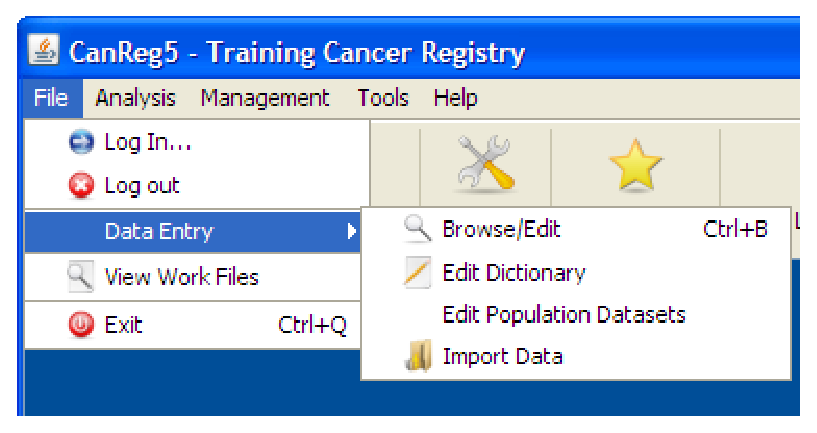
\includegraphics[width=3.91667in,height=2in]{17}
\par\end{center}
\begin{itemize}
\item \begin{flushleft}
Click on {}``Import complete dictionary from file''.
\par\end{flushleft}
\end{itemize}
\begin{center}
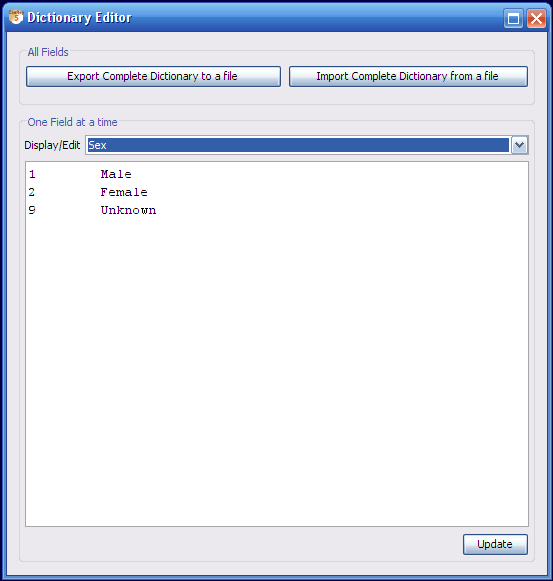
\includegraphics[width=4.79792in,height=5.04097in]{18}
\par\end{center}
\begin{itemize}
\item \begin{flushleft}
Browse and select the dictionary from you CanReg4 work folder or elsewhere. 
\par\end{flushleft}
\item \begin{flushleft}
Do Preview 
\par\end{flushleft}
\item \begin{flushleft}
Tick {}``CanReg4 Format'' if you are migrating from CanReg4, leave
unticked if you are using the demo system or otherwise are importing
a CanReg5 formatted dictionary.
\par\end{flushleft}
\end{itemize}
\begin{center}
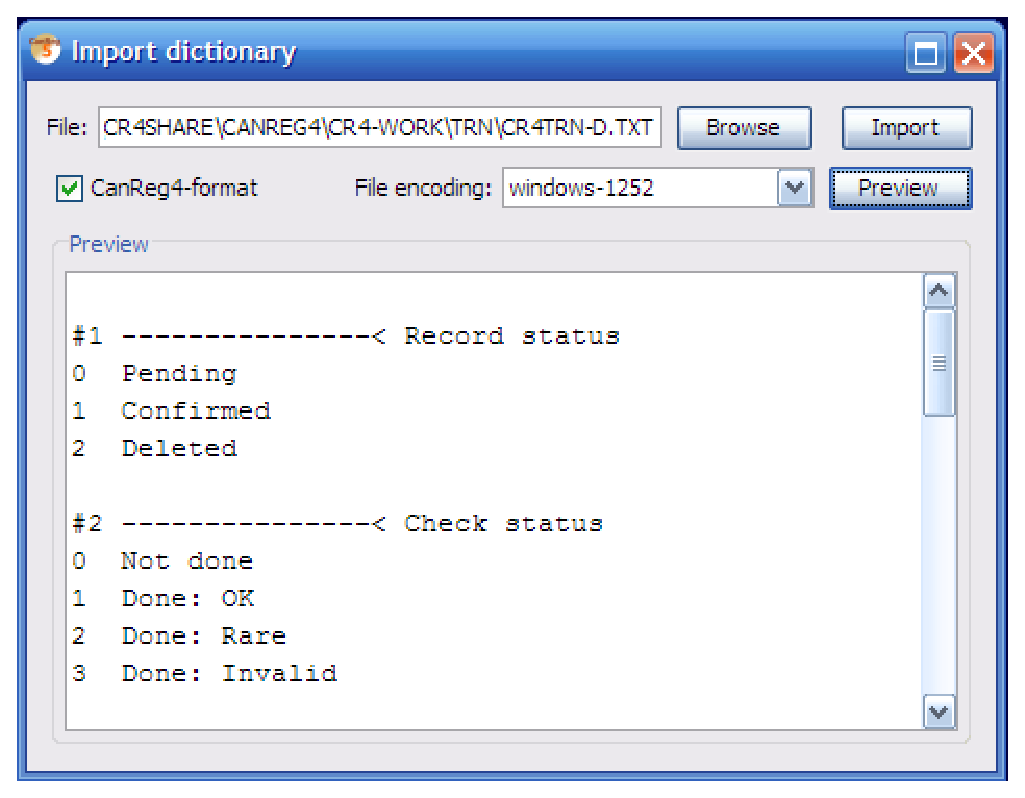
\includegraphics[width=4.95833in,height=3.82292in]{19}
\par\end{center}
\begin{itemize}
\item \begin{flushleft}
Click Import. This might take some time. Please note the bar in the
lower right indicating that the program is busy. 
\par\end{flushleft}
\item \begin{flushleft}
Afterwards you will receive a message of success imported. 
\par\end{flushleft}
\item \begin{flushleft}
Click OK. 
\par\end{flushleft}
\item \begin{flushleft}
Go back to {}``File'', {}``Data Entry'', {}``Edit dictionary''
and verify that the dictionaries have been imported. 
\par\end{flushleft}
\end{itemize}

\subsection{\textsf{Import the data from CanReg4}}

\begin{flushleft}
Make sure to export the most updated data from your CanReg4 system. 
\par\end{flushleft}
\begin{itemize}
\item \begin{flushleft}
In CanReg4: {}``Analysis'', {}``Export data'' 
\par\end{flushleft}
\item \begin{flushleft}
Tick {}``Export all variables''. 
\par\end{flushleft}
\item \begin{flushleft}
Choose variables names short 
\par\end{flushleft}
\item \begin{flushleft}
\textbf{Under {}``Export File options'' choose {}``Comma separated
variables''} 
\par\end{flushleft}
\item \begin{flushleft}
Untick {}``Format date'' 
\par\end{flushleft}
\item \begin{flushleft}
Untick {}``Correct Unknown'' 
\par\end{flushleft}
\item \begin{flushleft}
Click {}``write data to file'' and pick a file name that you can
find back easily in CanReg5. For example on the desktop. Click {}``save''. 
\par\end{flushleft}
\item \begin{flushleft}
Take a look at the data you have now exported and close CanReg4. 
\par\end{flushleft}
\item \begin{flushleft}
Back in CanReg5 do {}``File'', {}``Data Entry'' and {}``Import
Data''.
\par\end{flushleft}
\end{itemize}
\begin{center}
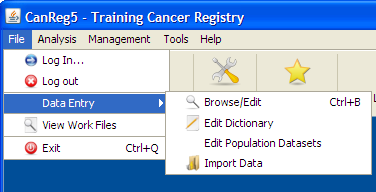
\includegraphics[width=3.91667in,height=2in]{20}
\par\end{center}
\begin{itemize}
\item \begin{flushleft}
The program will ask you if you have all your data in one file. Answer
{}``yes'' as this is the case when migrating from CanReg4. 
\par\end{flushleft}
\item \begin{flushleft}
Click {}``Browse'' and locate the file from step A. Select it and
click {}``Open''. You can if you want preview the file to see that
you picked the right one and that the file looks OK. If for example
Arabic names are garbled you should try to choose another {}``File
encoding'' (Default for Arabic text is ISO-8859-6). 
\par\end{flushleft}
\item \begin{flushleft}
\textbf{Set {}``Separating character'' to Comma.} (Or whatever separating
characters your file has.)
\par\end{flushleft}
\end{itemize}
\begin{center}
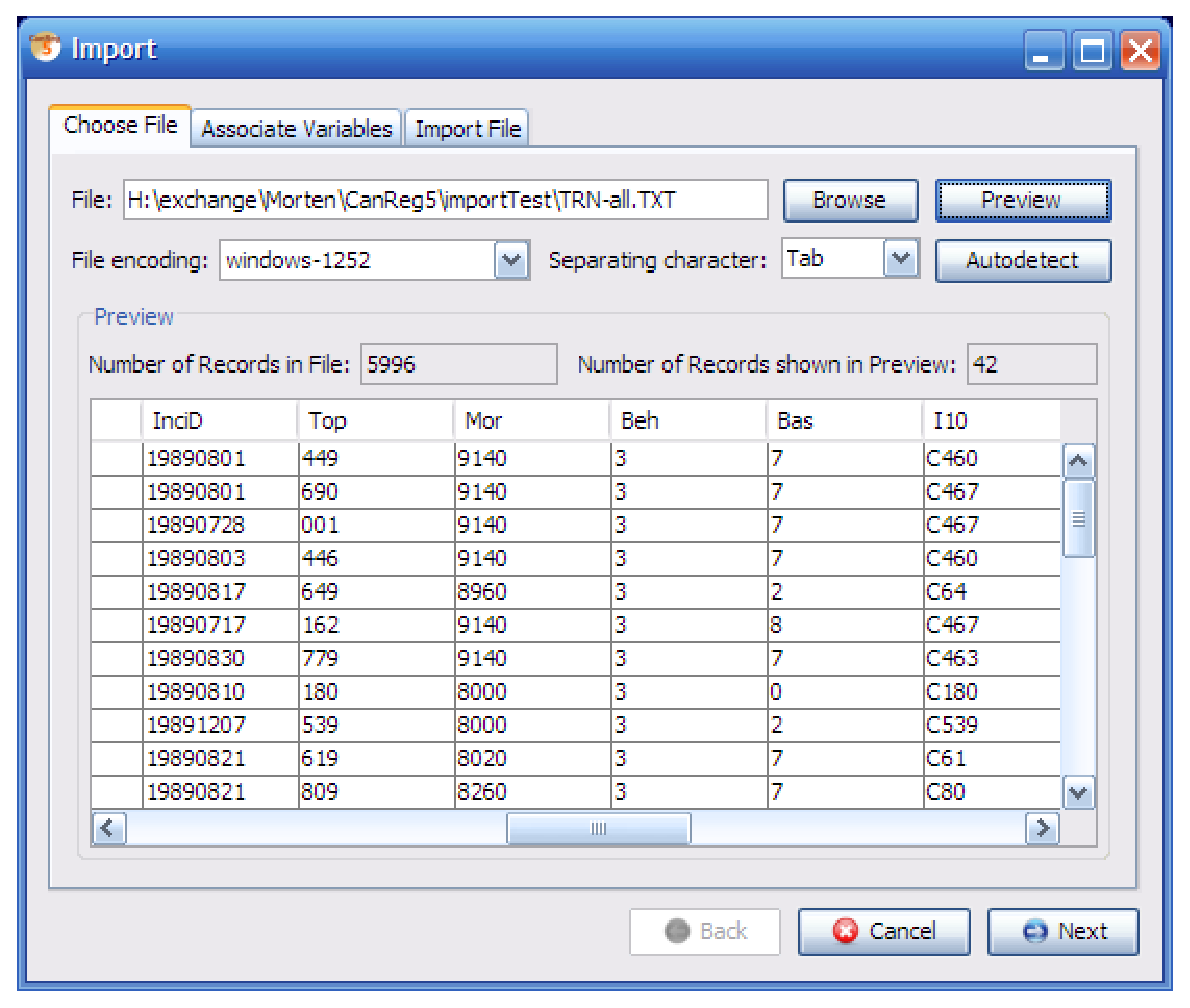
\includegraphics[width=5.00069in,height=4.21667in]{21}
\par\end{center}
\begin{itemize}
\item \begin{flushleft}
Click Preview to see that the data looks OK. 
\par\end{flushleft}
\item \begin{flushleft}
Click {}``Next'' (or select the tab {}``Associate Variables'') 
\par\end{flushleft}
\item \begin{flushleft}
This lets you associate the variables in the file to import with the
variables in the database. CanReg5 will find most of these associations
by itself, but you should revise them to see if they look OK. Look
for variable names in bold, as they are the one that are not assigned
at all. 
\par\end{flushleft}
\item \begin{flushleft}
Click {}``Next'' (or select the tab {}``Import File'') 
\par\end{flushleft}
\item \begin{flushleft}
Click {}``Import'' (leave everything as by default -- the import
function only works on empty CanReg databases as per now\ldots{}) 
\par\end{flushleft}
\item \begin{flushleft}
Let CanReg5 import the data (this might take a while) and click {}``OK''. 
\par\end{flushleft}
\item \begin{flushleft}
Click {}``Browse/Edit'' and {}``Refresh Table'' to see that the
data has arrived well. 
\par\end{flushleft}
\end{itemize}

\subsection{\textsf{Import data from other programs}}

\begin{flushleft}
You can import data from other programs than CanReg4 by using the
import tool in CanReg5. The only thing to pay attention to is that
the data has to be coded in exactly the same way as in the CanReg5
database. 
\par\end{flushleft}
\begin{itemize}
\item \begin{flushleft}
Dates should be coded as year month day (yyyyMMdd)
\par\end{flushleft}
\item \begin{flushleft}
Topography in 3 digits ICD-O-3 with no leading C.
\par\end{flushleft}
\item \begin{flushleft}
Morphology in 4 (or 5) digits ICD-O-3.
\par\end{flushleft}
\end{itemize}
\begin{flushleft}
Other fields with dictionaries, like for example addresses should
follow the dictionary defined for them in CanReg5. 
\par\end{flushleft}

\begin{flushleft}
The data can either be in a single file as the example for CanReg4,
or in one separate file for patient-information, tumour information
and source information (with pointers to link sources to tumours and
tumours to patients). 
\par\end{flushleft}


\section{Working with CanReg5}


\subsection{\textsf{Back up and restore}}

\begin{flushleft}
Backup-functionality can be found under the Management menu. 
\par\end{flushleft}


\subsubsection{Perform backup }

\begin{flushleft}
Under {}``Management'' click {}``Backup''
\par\end{flushleft}

\begin{center}
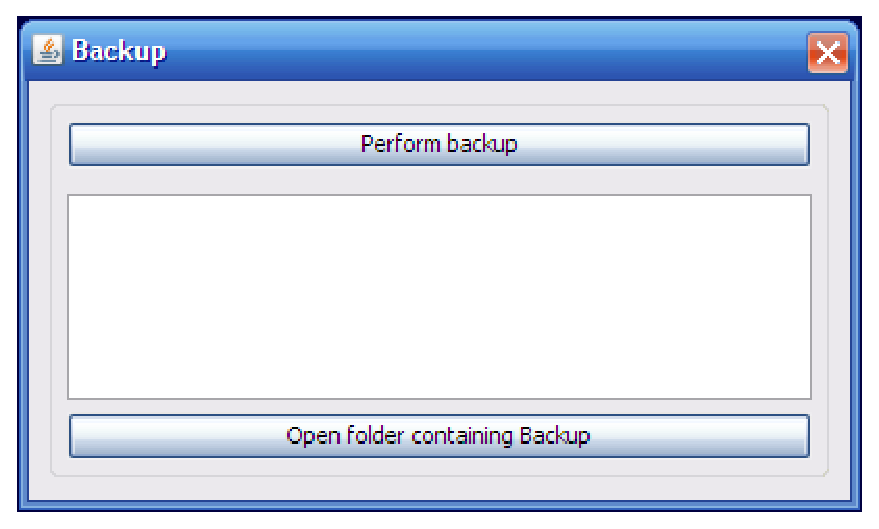
\includegraphics[width=4.22917in,height=2.47917in]{22}
\par\end{center}

\begin{flushleft}
Then click {}``Perform backup''. This creates the backup of the
CanReg5 database on the server machine. If you are on the server machine,
you can see the files you created by clicking {}``Open folder containing
Backup''. It is stored in the \textbf{CanReg server} folder under
Backup and 3 digit code of the registry and then the date of the backup.
On my machine, for example, it is {}``C:\textbackslash{}Documents
and Settings\textbackslash{}morten\textbackslash{}.CanRegServer\textbackslash{}Backup\textbackslash{}TRN\textbackslash{}2009-01-14''. 
\par\end{flushleft}


\subsubsection{Restore from backup }

\begin{flushleft}
If you are on the server machine you can restore the backup you created
above by clicking {}``Restore'' in the {}``Management''-menu and
choose the folder with the date of the backup you want to restore
- either by entering it or by browsing for it.
\par\end{flushleft}

\begin{center}
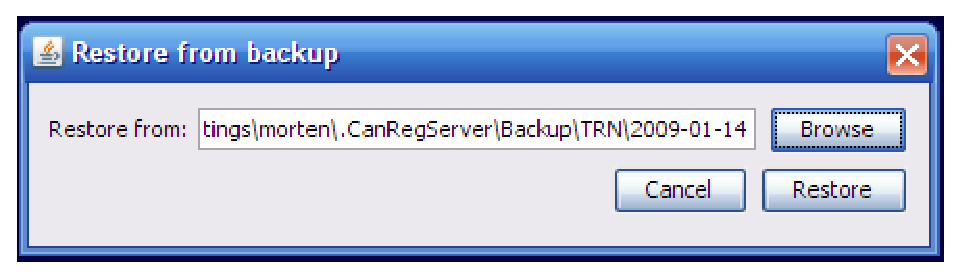
\includegraphics[width=4.63542in,height=1.22917in]{23}
\par\end{center}


\subsection{\textsf{Enter cases}}

\begin{flushleft}
To get to a data entry form either press Create New Record from the
menu bar
\par\end{flushleft}

\begin{center}
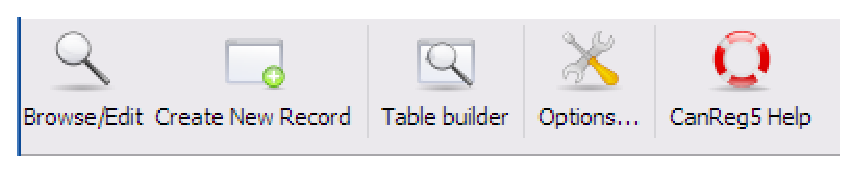
\includegraphics[width=4.11458in,height=0.697917in]{24} 
\par\end{center}

\begin{flushleft}
or enter a new record number in the browser and click {}``Edit Patient
ID:''
\par\end{flushleft}

\begin{center}
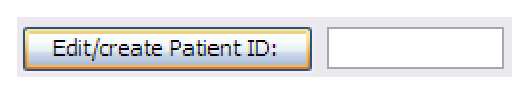
\includegraphics[width=2.47917in,height=0.302083in]{25}
\par\end{center}

\begin{flushleft}
This should resemble your CanReg4 data entry form, except that it
is split in a patient part and a tumour part with a source part. Another
thing to notice is the {}``Obsolete'' button. This will flag the
record as obsolete, so that it will not show up in analysis. It is
a way to keep duplicate records that might contain valuable information.
Pink fields are the mandatory ones. (Date format is still set to yyyyMMdd,
but this will be improved later.)
\par\end{flushleft}

\begin{center}
\includegraphics[scale=0.5]{\string"C:/Documents and Settings/ervikm/My Documents/NetBeansProjects/CanReg/doc/CanReg5-Instructions/DataEntryExample\string".eps}
\par\end{center}


\subsection{\textsf{Export data}}

\begin{flushleft}
To export your data go to Analysis -- Export Data/Reports:
\par\end{flushleft}

\begin{center}
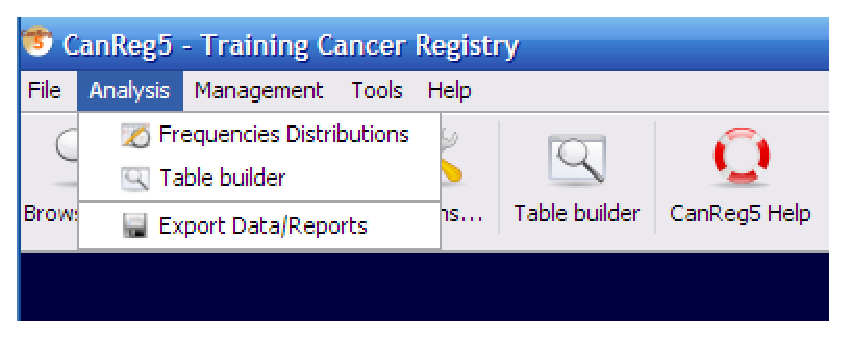
\includegraphics[width=4.0625in,height=1.52083in]{27}
\par\end{center}

\begin{flushleft}
You will be presented with a screen that resembles the browse-screen:
\par\end{flushleft}

\begin{center}
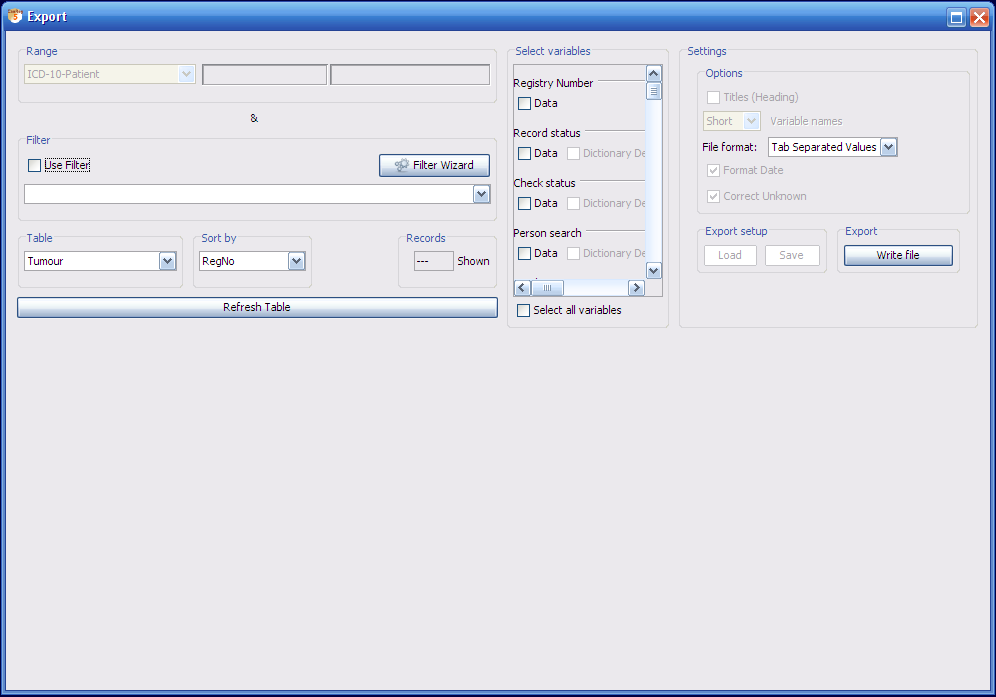
\includegraphics[width=5.4785in,height=4.0292in]{28}
\par\end{center}

\begin{flushleft}
Now you can select some variables, and tables and sort method and
export (some of) your data. Please note that some of the functionality,
like the ability to store export-setups is not yet implemented. 
\par\end{flushleft}

\begin{flushleft}
If you export data to a {}``Tab Separated'' file you can open this
in general spreadsheets (like Excel). 
\par\end{flushleft}


\subsection{\textsf{Manage users}}

\begin{flushleft}
The user manager is located under management -- users:
\par\end{flushleft}

\begin{center}
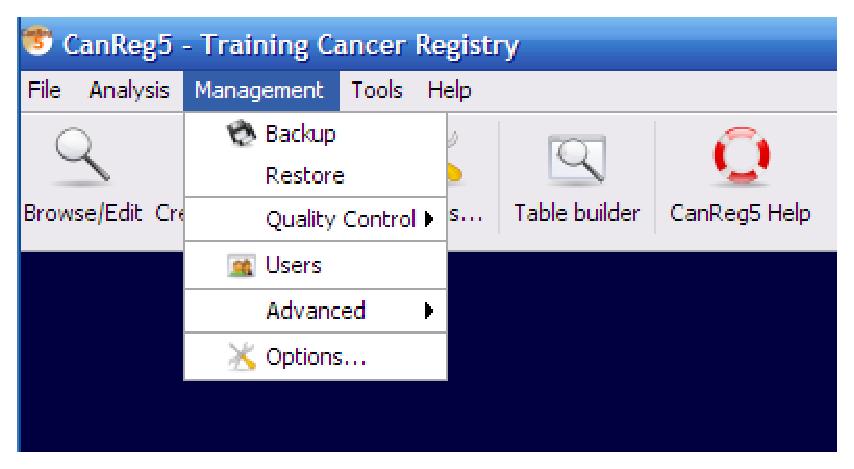
\includegraphics[width=4.10417in,height=2.17708in]{29}
\par\end{center}

\begin{flushleft}
\textbf{Change your own password} 
\par\end{flushleft}

\begin{flushleft}
To change your own password, go to the Current user tab in the user
manager and enter your new password twice:
\par\end{flushleft}

\begin{center}
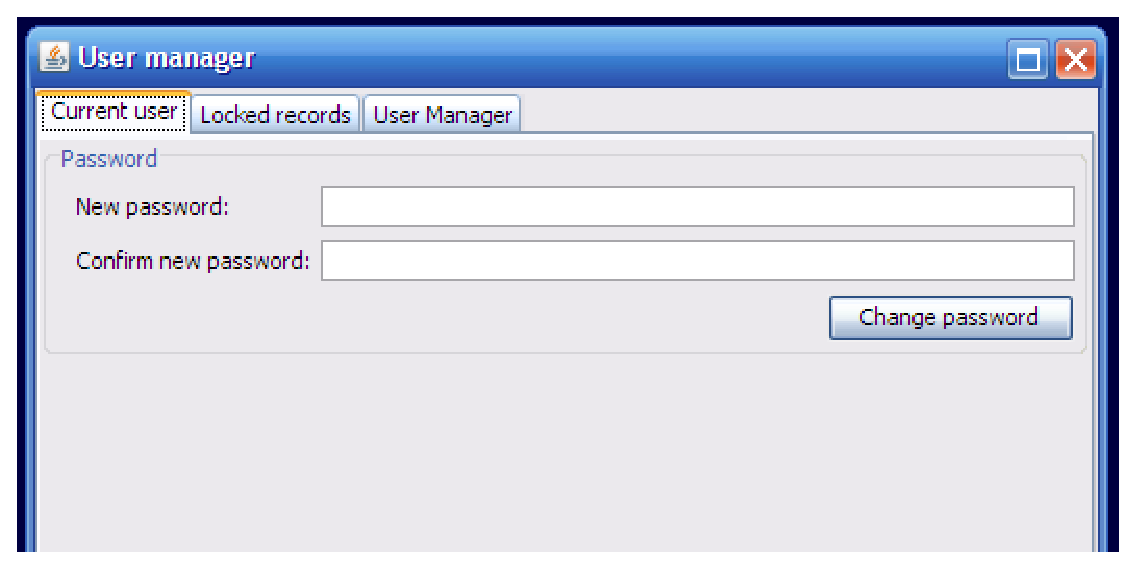
\includegraphics[width=5.4785in,height=2.6764in]{30} 
\par\end{center}

\begin{flushleft}
\textbf{Locked records} 
\par\end{flushleft}

\begin{flushleft}
Not yet implemented. 
\par\end{flushleft}

\begin{flushleft}
\textbf{User manager} 
\par\end{flushleft}

\begin{flushleft}
If you are logged in with Supervisor rights you have access to the
User manager part of the user manager. This allows you to add and
delete users.
\par\end{flushleft}

\begin{center}
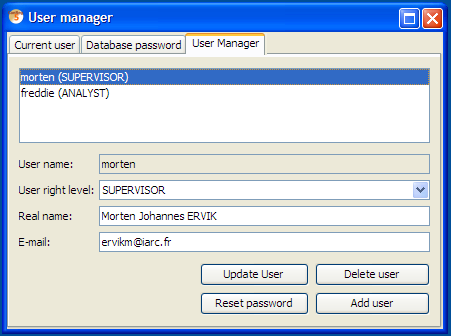
\includegraphics[width=4.64583in,height=3.70833in]{31}
\par\end{center}

\begin{flushleft}
The default password of any user is its user name. 
\par\end{flushleft}


\subsection{\textsf{Population Dataset Editor}}

\begin{flushleft}
The Population Dataset editor lets you edit population data set to
be used in the table builder. This is located under File -- Data Entry
Edit Population Dataset: 
\par\end{flushleft}

\begin{center}
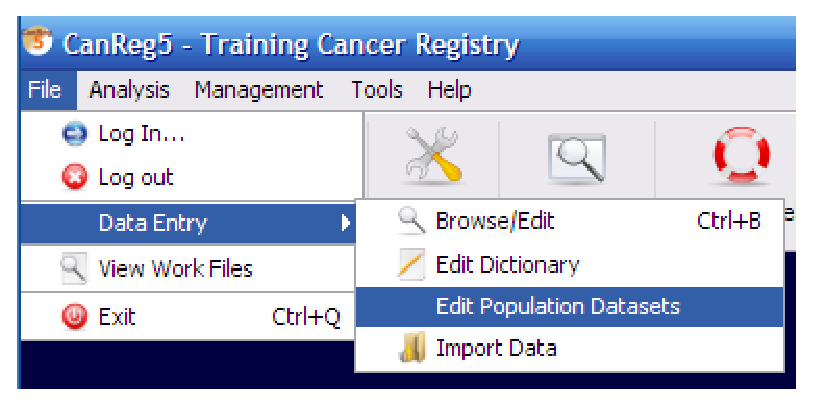
\includegraphics[width=3.89583in,height=1.86458in]{32}
\par\end{center}

\begin{flushleft}
When you start it you get to the list of all your population datasets.
\par\end{flushleft}

\begin{center}
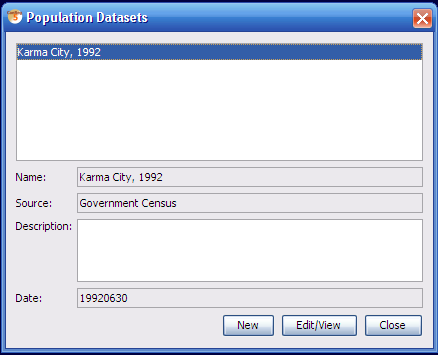
\includegraphics[width=4.5625in,height=3.69792in]{33}
\par\end{center}

\begin{flushleft}
Add one by clicking New. This opens the Population Dataset editor: 
\par\end{flushleft}

\begin{center}
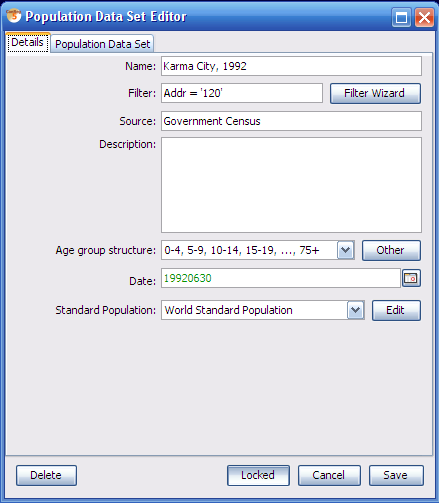
\includegraphics[width=4.57292in,height=5.23958in]{34}
\par\end{center}

\begin{flushleft}
Fill in the details:
\par\end{flushleft}
\begin{itemize}
\item \begin{flushleft}
A name for the dataset 
\par\end{flushleft}
\item \begin{flushleft}
A filter if it does not cover your entire area of your database. 
\par\end{flushleft}
\item \begin{flushleft}
A source 
\par\end{flushleft}
\item \begin{flushleft}
Some description (less than 255 characters) 
\par\end{flushleft}
\item \begin{flushleft}
Choose the age group structure. 
\par\end{flushleft}
\item \begin{flushleft}
Set the date of the population dataset. (In the example above it is
mid 1992) 
\par\end{flushleft}
\item \begin{flushleft}
The Standard population used for ASRs when building tables with this
set. 
\par\end{flushleft}
\end{itemize}
\begin{flushleft}
Then fill the population dataset itself: 
\par\end{flushleft}

\begin{center}
\includegraphics{\string"C:/Documents and Settings/ervikm/My Documents/NetBeansProjects/CanReg/doc/CanReg5-Instructions/CanRegPopSetEditor\string".eps}
\par\end{center}

\begin{flushleft}
(Please note that you can copy and paste population datasets back
and forth from general spreadsheets like Excel.) 
\par\end{flushleft}

\begin{flushleft}
Click save to save your population dataset. 
\par\end{flushleft}


\subsubsection{Import population data set from CanReg4 }

\begin{flushleft}
Alternatively you can import population data sets from CanReg4. To
do this you go to the Tools menu and choose {}``Load CanReg4 Population
Dataset''.
\par\end{flushleft}

\begin{center}
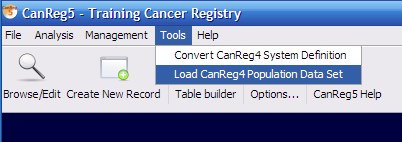
\includegraphics[width=4.1875in,height=1.47917in]{36}
\par\end{center}

\begin{flushleft}
Click Browse to find the population dataset:
\par\end{flushleft}

\begin{center}
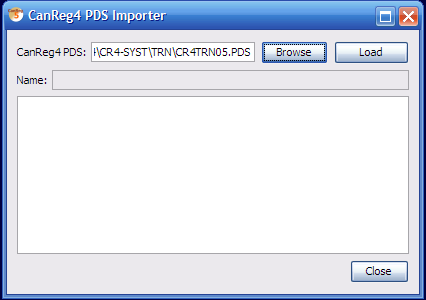
\includegraphics[width=4.4375in,height=3.125in]{37}
\par\end{center}

\begin{flushleft}
Then click Load and a confirmation message that the population dataset
has been loaded will appear.
\par\end{flushleft}

\begin{center}
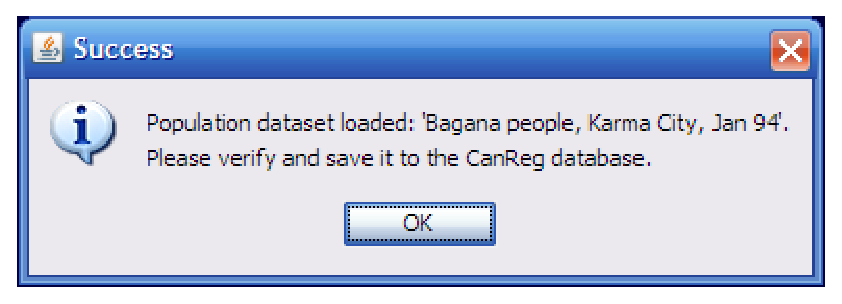
\includegraphics[width=4.04167in,height=1.35417in]{38}
\par\end{center}

\begin{flushleft}
Click {}``OK''. 
\par\end{flushleft}

\begin{flushleft}
Next step is to revise the population dataset and see to that it has
been imported correctly.
\par\end{flushleft}

\begin{center}
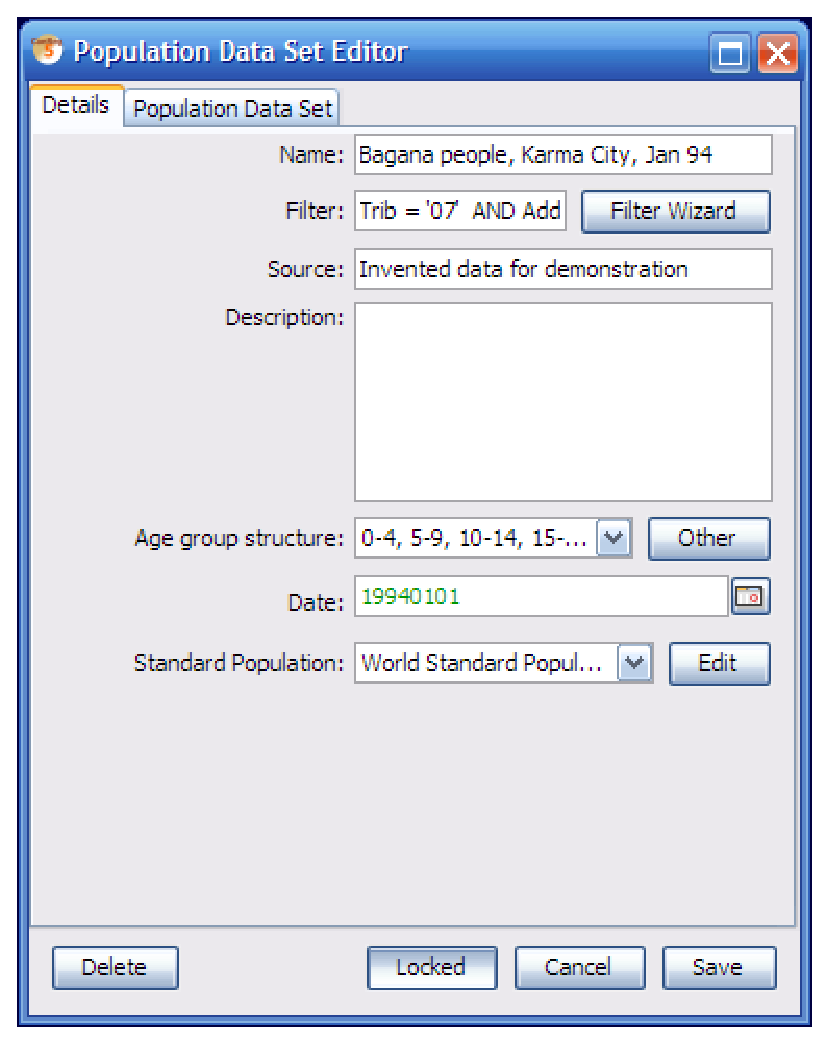
\includegraphics[width=3.97917in,height=5.05208in]{39} 
\par\end{center}

\begin{flushleft}
One important thing to do is to see to that the filter is correct.
That for example the search variables are enclosed by 's. If you need
to change anything in the dataset you need to unlock it by toggling
the {}``Locked''-toggle. 
\par\end{flushleft}


\subsection{\textsf{Table builder}}

\begin{flushleft}
The Table builder lets you build incidence tables etc in CanReg. You
find it under analysis -- table builder. 
\par\end{flushleft}

\begin{center}
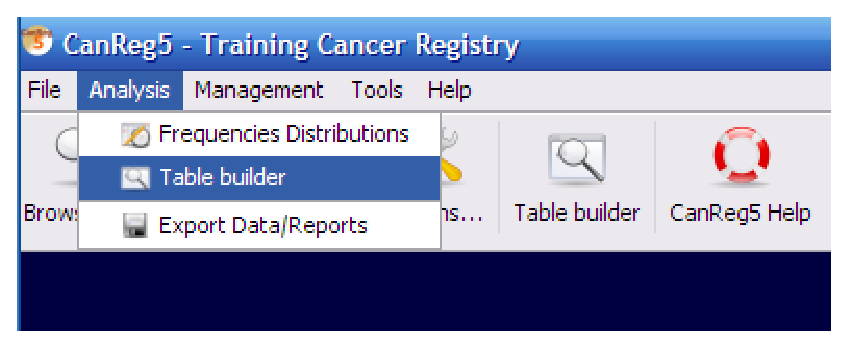
\includegraphics[width=4.07292in,height=1.57292in]{40}
\par\end{center}

\begin{flushleft}
When you start it you first choose the type of table you want to produce.
(Please note that it is only the Incidence per 100,000 by age group
(period) and the Population pyramid that is implemented so far\ldots{})
Pick Incidence per 100,000 by age group (Period): 
\par\end{flushleft}

\begin{center}
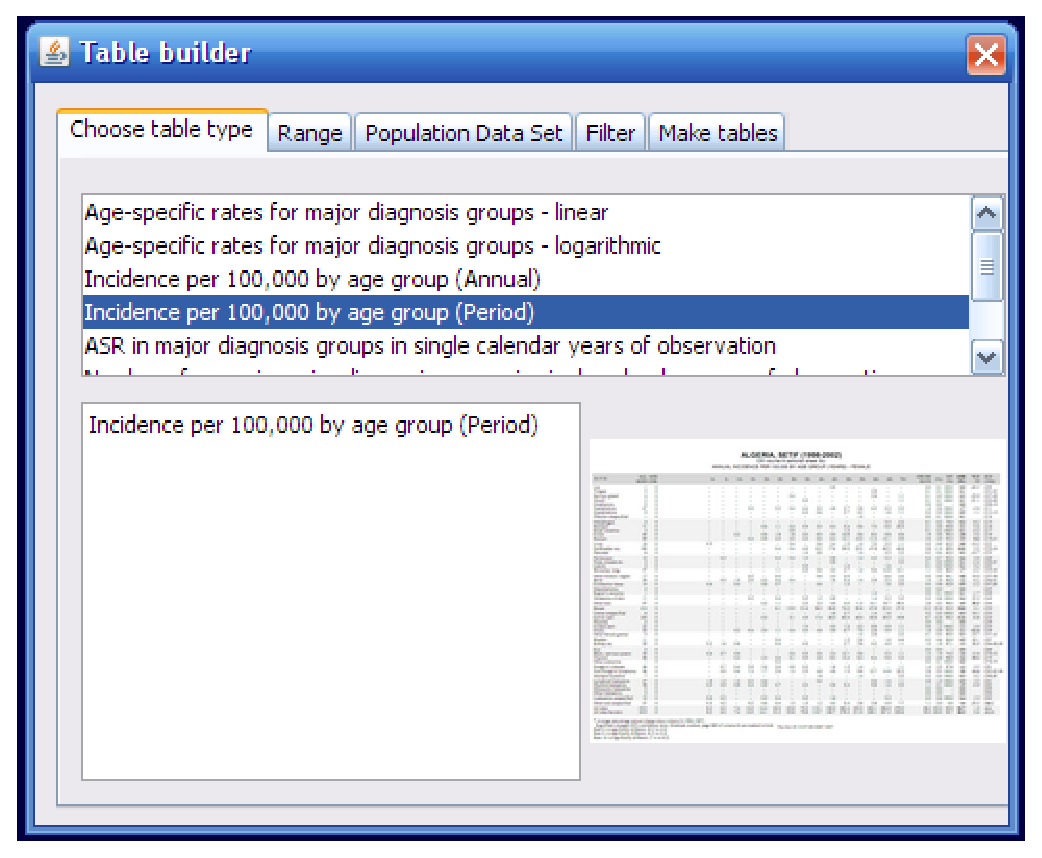
\includegraphics[width=5.04167in,height=4.125in]{41}
\par\end{center}

\begin{flushleft}
Then click on range to set the range of your analysis and set it to
match the analysis you want to do, for example here we want to look
at Karma City, 1991 to 1993: 
\par\end{flushleft}

\begin{center}
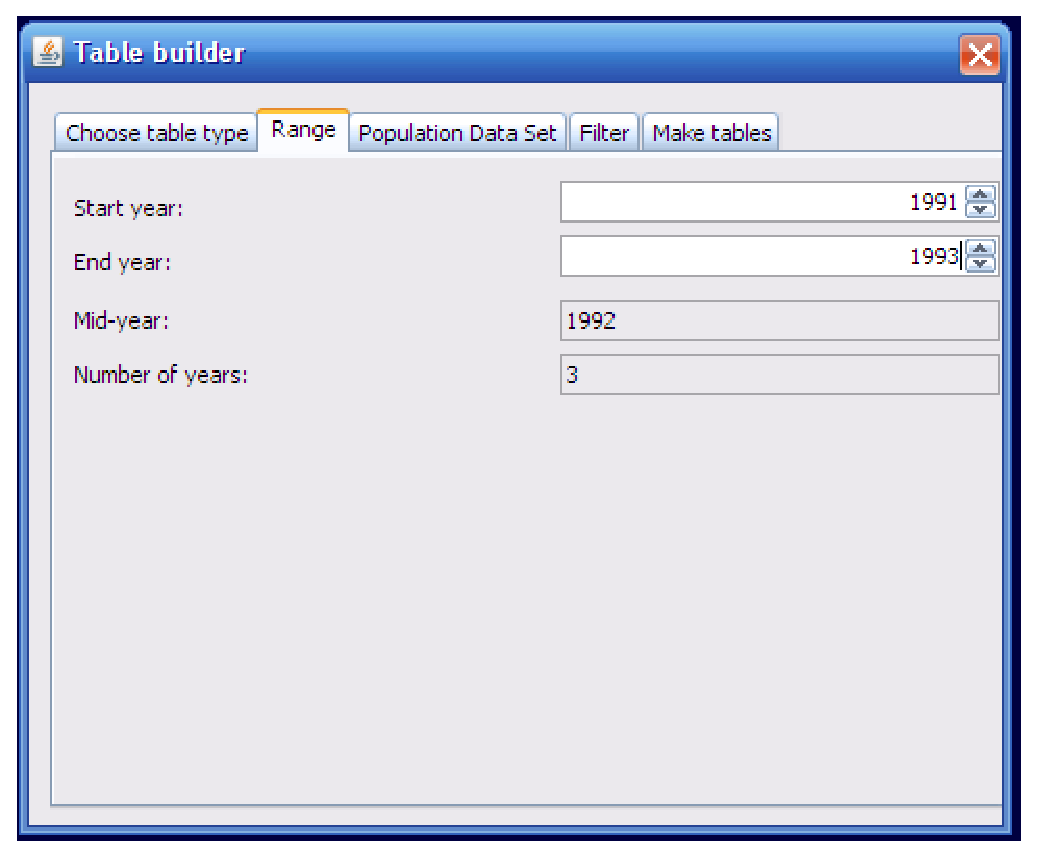
\includegraphics[width=5.02083in,height=4.125in]{42}
\par\end{center}

\begin{flushleft}
Click Population Data Set. Pick one population data set per year.
This can be the same for all three if that year is representative
of the period: 
\par\end{flushleft}

\begin{center}
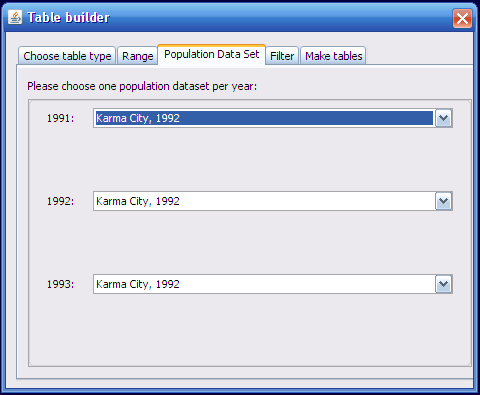
\includegraphics[width=5in,height=4.11458in]{43}
\par\end{center}

\begin{flushleft}
Then you can go to the Make tables tab to generate the actual tables.
Click {}``Generate post script files'' and choose a file name. (If
the table generates more than one file (like it is the case for incidence
per 100,000 some number or text will be added to the name you give
for each file.) 
\par\end{flushleft}

\begin{center}
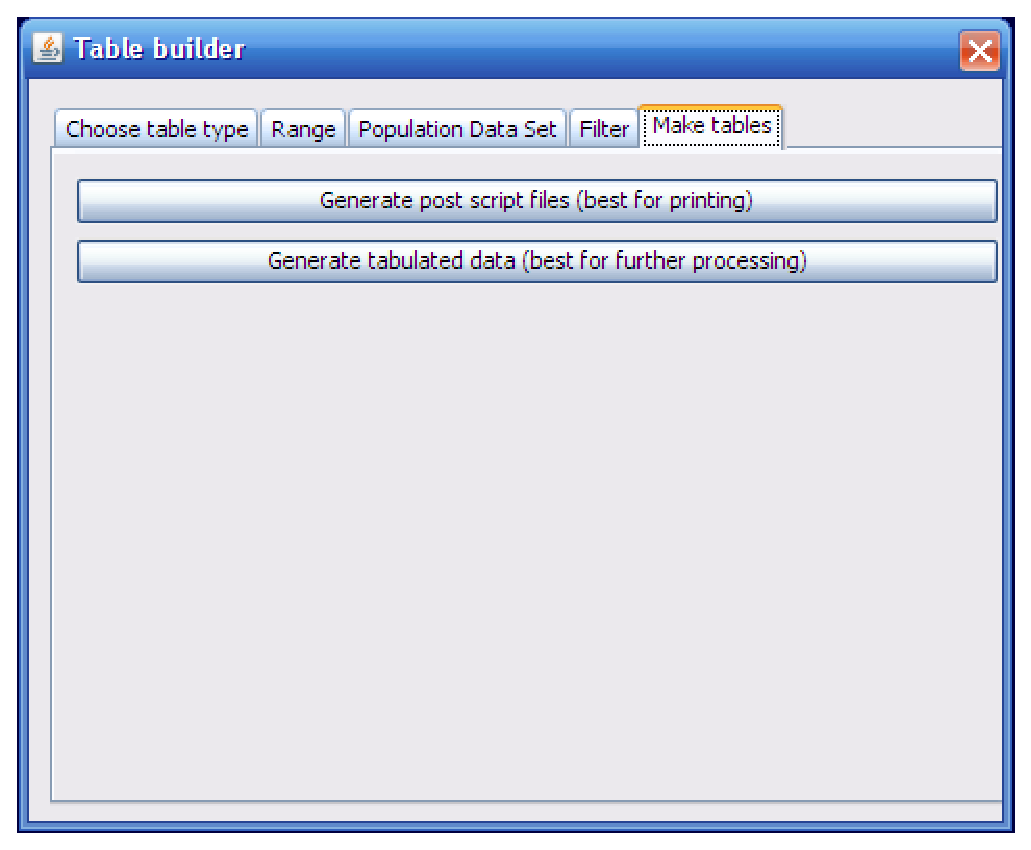
\includegraphics[width=4.98958in,height=4.08333in]{44} 
\par\end{center}

\begin{flushleft}
You get a message saying, {}``Tables built.'' 
\par\end{flushleft}

\begin{center}
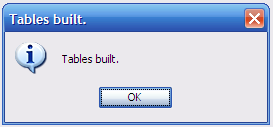
\includegraphics[width=2.84375in,height=1.32292in]{45}
\par\end{center}

\begin{flushleft}
Click OK and if you have a program that can read PostScript (See page
\pageref{sub:Tables}.) files the tables will be displayed after you
press OK. 
\par\end{flushleft}

\begin{center}
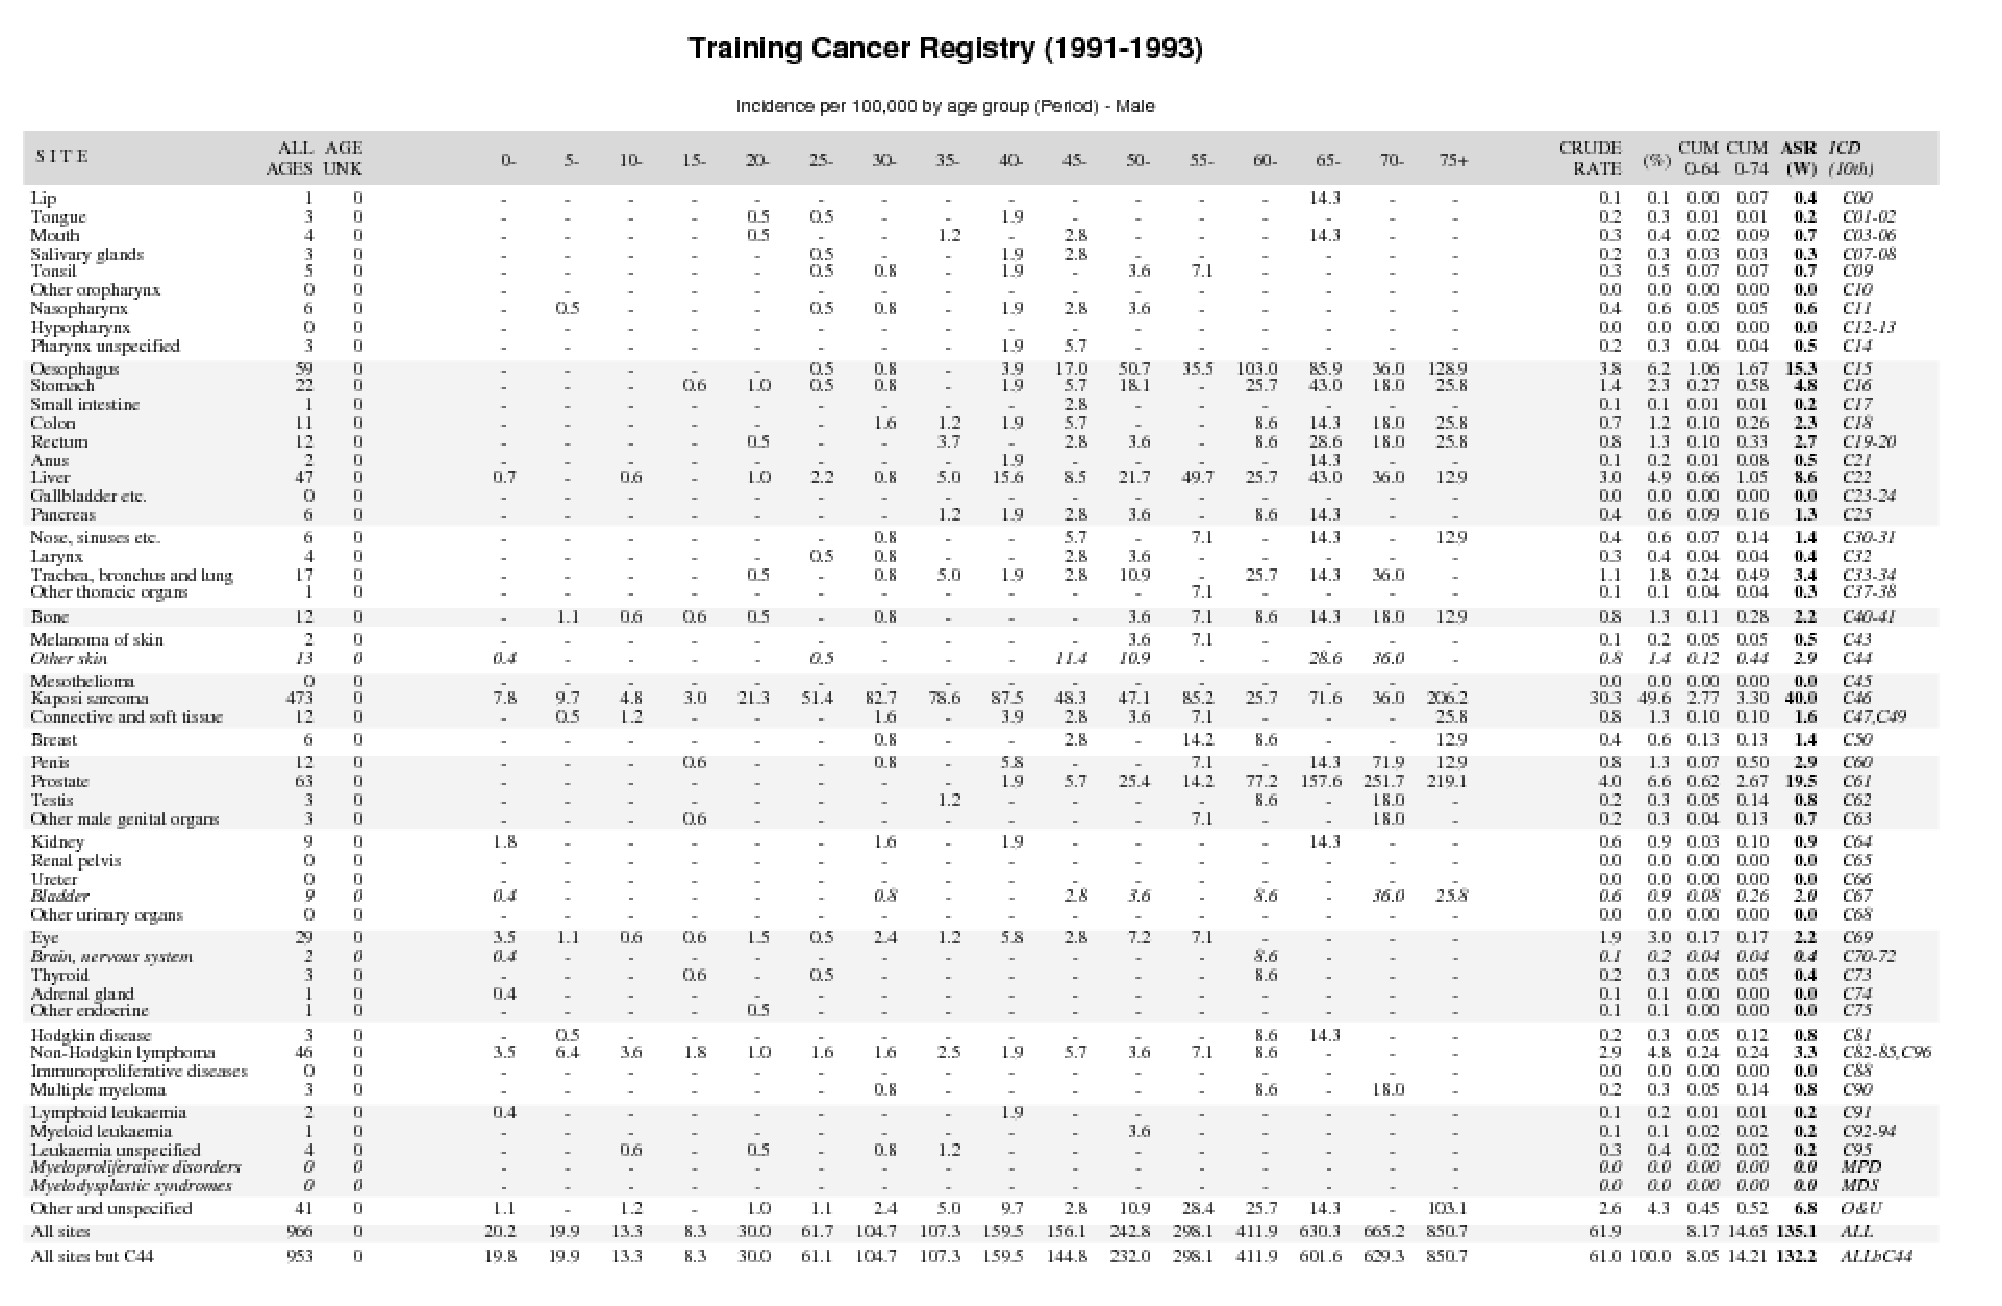
\includegraphics[width=5.4785in,height=3.7229in]{46}
\par\end{center}


\subsection{\textsf{Frequency distributions}}

\begin{flushleft}
Frequencies distributions let you look at the data in your database
as frequencies by year. You can cross-tabulate several variables.
To start this module go to Analysis -- Frequencies Distributions: 
\par\end{flushleft}

\begin{center}
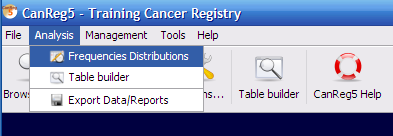
\includegraphics[width=4.09375in,height=1.41667in]{47}
\par\end{center}

\begin{flushleft}
If you click Refresh table with no filter and no selected variables
you get a table of cases per year. 
\par\end{flushleft}

\begin{center}
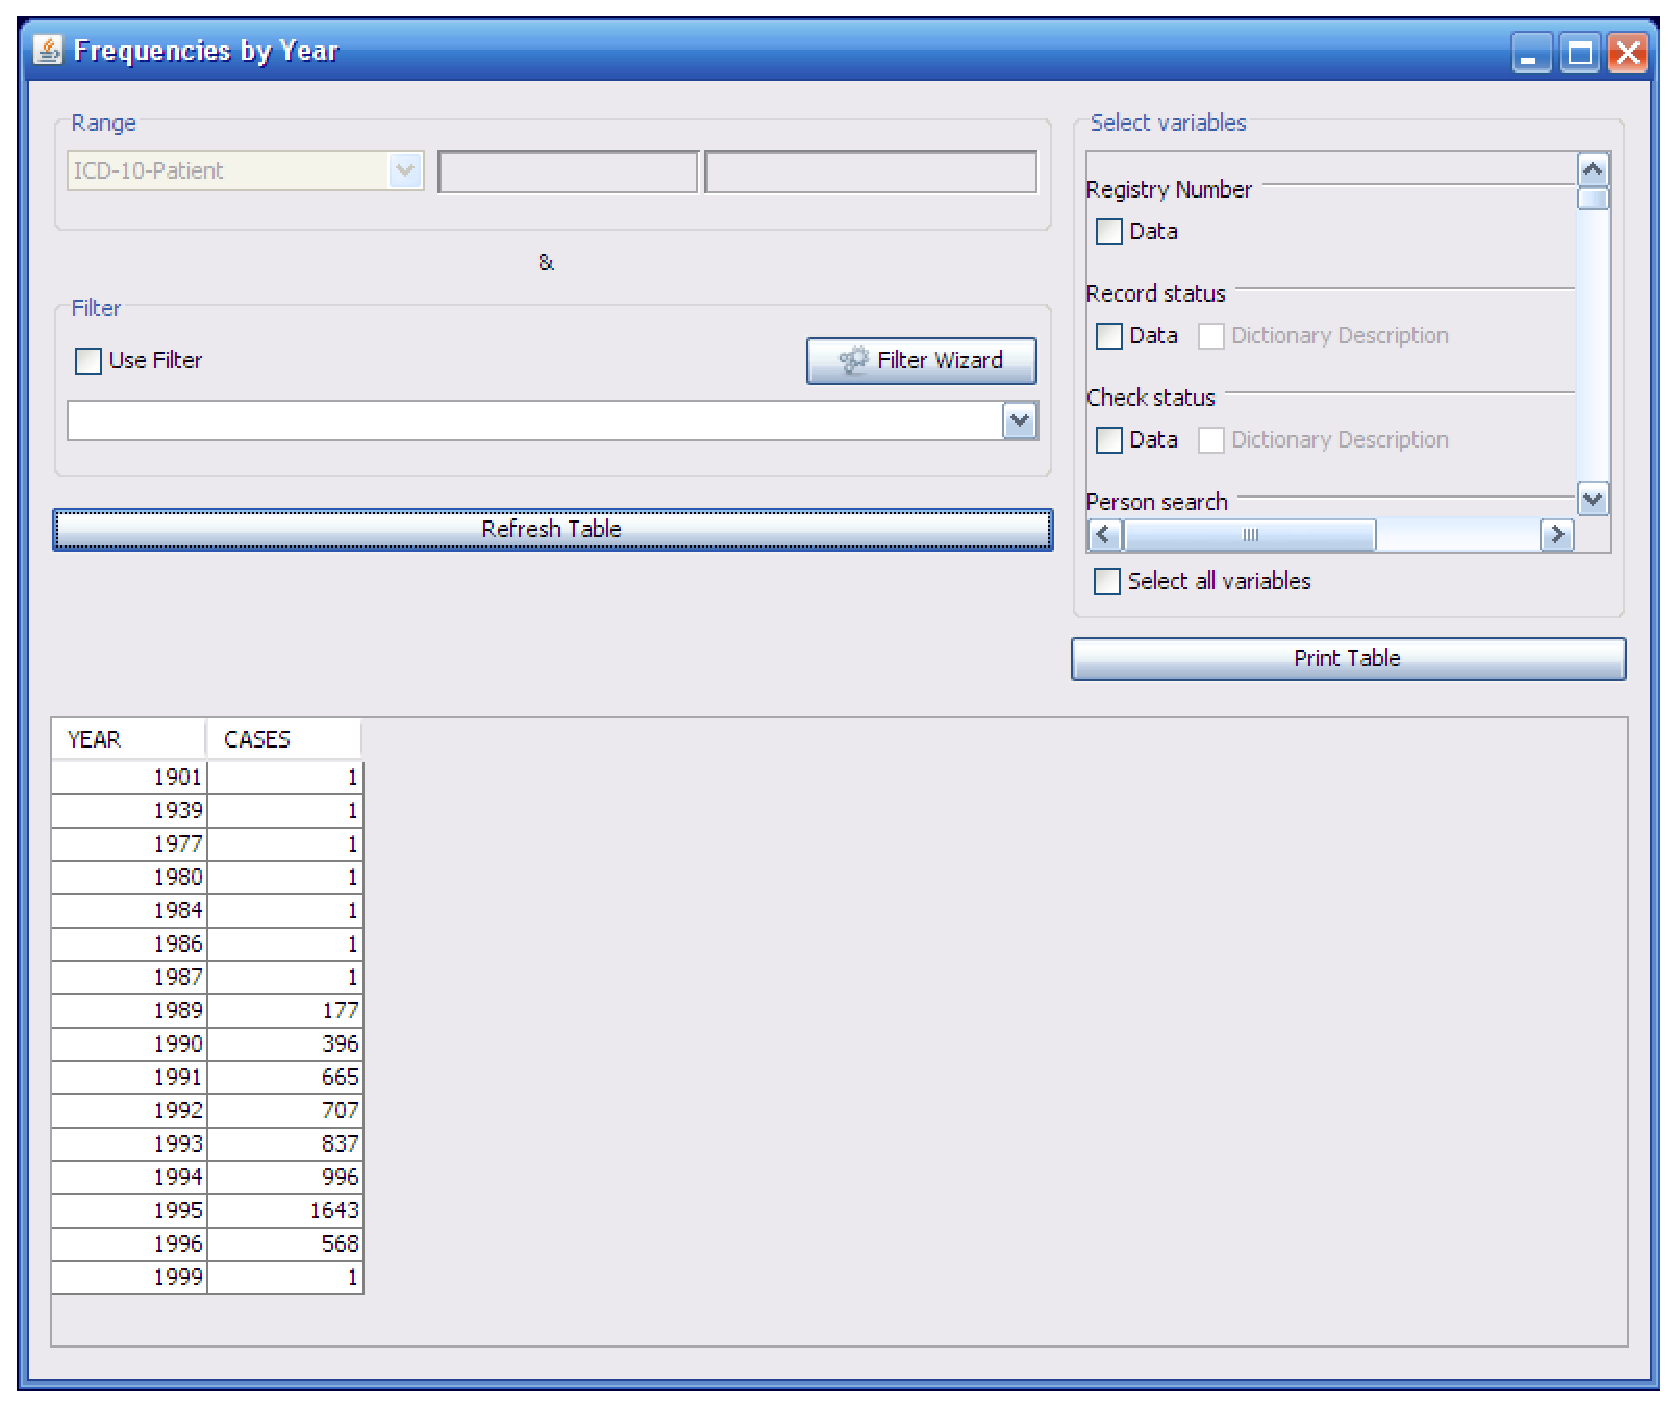
\includegraphics[width=5.4785in,height=4.8181in]{48}
\par\end{center}

\begin{flushleft}
You can sort by any field by clicking its header. For example by number
of cases: 
\par\end{flushleft}

\begin{center}
\includegraphics[width=1.60417in,height=2.94792in]{49}
\par\end{center}

\begin{flushleft}
You can filter the result by adding a filter like for example on incidence
date. You can also add as many variables as you want. 
\par\end{flushleft}

\begin{center}
\includegraphics[width=5.4785in,height=4.8042in]{50} 
\par\end{center}

\begin{flushleft}
This table can be selected and copied and pasted into Excel, for example.
(No right-click shortcut for that is implemented yet, but you can
select the lines you want and press Ctrl-C (on Windows and Linux)
or Apple-C (on Mac) and paste it into other programs. 
\par\end{flushleft}

\appendix

\section{\textsf{Frequently asked questions (FAQ)}}


\subsection{Server }
\begin{description}
\item [{Q:}] \begin{flushleft}
When I click the {}``Launch Server''/{}``Test Connection''
button, it takes \textbf{more than 3 minutes} to launch the server
and I get the message that the {}``Server {[}is{]} already running''.
Afterwards I cannot log in. 
\par\end{flushleft}
\item [{A:}] \begin{flushleft}
Xenios found the following solution: On our PCs, we use Microsoft
Internet Explorer 7. In the {}``Tools / Internet Options / Connections
/ LAN Settings'' we have a tick in the checkbox for {}``Use a proxy
server for your LAN'' and the address and port of the proxy server
filled in accordingly. I put a tick in the checkbox for {}``Bypass
proxy server for local addresses'', clicked the {}``Advanced''
button and typed the IP address of the PC (localhost) in the {}``Do
not use proxy server for addresses beginning with:'' box. 
\par\end{flushleft}
\end{description}

\subsection{Conversion CanReg4 to CanReg5}
\begin{description}
\item [{Q:}] \begin{flushleft}
In what table should the variable age be stored?
\par\end{flushleft}
\item [{A:}] \begin{flushleft}
The tumour table. Like that, if the same patient has a new
tumour you can (probably) keep the patient record and just add a new
tumour record. Birth date is stored in the patient table. (Incidence
date with the tumour.) 
\par\end{flushleft}
\item [{Q:}] \begin{flushleft}
Do I need to {}``install'' the CanReg5 system definition
file after converting from CanReg4 using the built in tool? 
\par\end{flushleft}
\item [{A:}] \begin{flushleft}
After converting the system you don't need to {}``install''
it afterwards as the XML file is automatically copied to your system
folder during conversion. 
\par\end{flushleft}
\item [{Q:}] \begin{flushleft}
I get errors during import of the data from CanReg4. The process
stops after a certain percentage every time. 
\par\end{flushleft}
\item [{A:}] \begin{flushleft}
Try exporting your data with a comma separated variables instead
of the default tab-separated ones (or vice versa) and see if that
helps. 
\par\end{flushleft}
\end{description}

\subsection{Dictionary}
\begin{description}
\item [{Q:}] \begin{flushleft}
Can I import dictionaries from other CanReg systems to my
own? 
\par\end{flushleft}
\item [{A:}] \begin{flushleft}
Since most CanReg systems have different dictionary structure
(length of codes, order of dictionaries etc.) you need to import the
dictionary corresponding to your system or do necessary modifications. 
\par\end{flushleft}
\end{description}

\subsection{\label{sub:Tables}Tables}
\begin{description}
\item [{Q:}] \begin{flushleft}
What program can I use to view the postscript files with? 
\par\end{flushleft}
\item [{A:}] \begin{flushleft}
PostScript is an open standard, so you can use many different
tools to view them. (You can in many cases even send them directly
to a printer.) Apple's OSX and most Linux-distributions (Ubuntu, RedHat,
SuSE etc) come with a tool to view them by default. On Windows the
tool I recommend is the open sourced and free GSview. (Available from:
\href{http://pages.cs.wisc.edu/~ghost/gsview/}{http://pages.cs.wisc.edu/$\sim$ghost/gsview/}
) To run GS View you need to install Ghostscript first. This can be
downloaded from here: \href{http://pages.cs.wisc.edu/~ghost/doc/GPL/gpl864.htm}{http://pages.cs.wisc.edu/$\sim$ghost/doc/GPL/gpl864.htm}
(Scroll all the way down, under the heading Microsoft windows and
download the {}``GPL Ghostscript 8.64 for 32-bit Windows (the common
variety)'' (\href{http://mirror.cs.wisc.edu/pub/mirrors/ghost/GPL/gs864/gs864w32.exe}{http://mirror.cs.wisc.edu/pub/mirrors/ghost/GPL/gs864/gs864w32.exe})
Run this file to install Ghostscript. Then you can get GS View from
here: \href{http://pages.cs.wisc.edu/~ghost/gsview/get49.htm}{http://pages.cs.wisc.edu/$\sim$ghost/gsview/get49.htm}
(Most probably, you should pick the Win32 self extracting archive
- the first download option. \href{http://mirror.cs.wisc.edu/pub/mirrors/ghost/ghostgum/gsv49w32.exe}{http://mirror.cs.wisc.edu/pub/mirrors/ghost/ghostgum/gsv49w32.exe})
Run this file to install GS View. 
\par\end{flushleft}
\end{description}

\subsection{Import}
\begin{description}
\item [{Q:}] \begin{flushleft}
Some letters are distorted/missing in records after an import.
(For example when importing Arabic names.) Why is that? 
\par\end{flushleft}
\item [{A:}] \begin{flushleft}
If the data is from a program that does not code the data
using Unicode (for example previous versions of CanReg) you need to
specify the coding scheme/{}``codepage'' during import of that file
to your database. If you pick the wrong one your data might get distorted.
To solve this problem you need to re-import the data. Please use the
preview button during import to see to that you have the right coding
scheme. 
\par\end{flushleft}
\end{description}

\section{Known issues}


\subsection{\textsf{Known bugs (errors)}}

\begin{flushleft}
Some known bugs: 
\par\end{flushleft}
\begin{itemize}
\item \begin{flushleft}
The result set in the browser is sometimes very slow to scroll around
in. 
\par\end{flushleft}

\begin{itemize}
\item \begin{flushleft}
Temporary solution: Use filters to minimize the number of records
shown at any time or only browse the {}``Patient'' or the {}``Tumour''
table. 
\par\end{flushleft}
\item \begin{flushleft}
Severity: Shouldn't cause loss of data 
\par\end{flushleft}
\item \begin{flushleft}
Priority: Low 
\par\end{flushleft}
\item \begin{flushleft}
Category: Database/Browser 
\par\end{flushleft}
\end{itemize}
\item \begin{flushleft}
Server does not start if language is set to Turkish due to special
rules in Turkish regarding {}``upper casing'' of letters. 
\par\end{flushleft}

\begin{itemize}
\item \begin{flushleft}
Temporary solution: set the language of the server to any other language
than Turkish. 
\par\end{flushleft}
\item \begin{flushleft}
Severity: Does not cause information loss 
\par\end{flushleft}
\item \begin{flushleft}
Priority: Medium 
\par\end{flushleft}
\item \begin{flushleft}
Category: Server 
\par\end{flushleft}
\end{itemize}
\end{itemize}

\subsection{\textsf{Known limitations}}
\begin{itemize}
\item \begin{flushleft}
Not all edit checks are in place? 
\par\end{flushleft}
\item \begin{flushleft}
Date fields not yet properly formatted. 
\par\end{flushleft}
\item \begin{flushleft}
You need a population dataset with 5 years age groups for many of
the tables to work properly\ldots{} 
\par\end{flushleft}
\item \begin{flushleft}
Age can not yet be calculated automatically. 
\par\end{flushleft}
\end{itemize}

\section{\textsf{Changelog}}


\subsubsection*{4.99.22 Build 858 }
\begin{itemize}
\item \begin{flushleft}
\texttt{Database engine switched to Java DB 10.5.3.0}\textbf{ }
\par\end{flushleft}
\item \begin{flushleft}
\texttt{RangeFilter now adds 's if needed by each variable.}\textbf{ }
\par\end{flushleft}
\item \begin{flushleft}
\texttt{Other bug fixes.}\textbf{ }
\par\end{flushleft}
\end{itemize}

\subsubsection*{4.99.21 Build 848 }
\begin{itemize}
\item \begin{flushleft}
\texttt{Access to handbook, possibility to download latest version.}\textbf{ }
\par\end{flushleft}
\item \begin{flushleft}
\texttt{DatabaseVariableEditor now throws error messages if somethings
not right with the variable definition during system setup.}\textbf{ }
\par\end{flushleft}
\item \begin{flushleft}
\texttt{ICCC3 converter implemented.}\textbf{ }
\par\end{flushleft}
\end{itemize}

\subsubsection*{4.99.20 }
\begin{itemize}
\item \begin{flushleft}
\texttt{Internationalization work. Portugese translation started. French
translation continued.} 
\par\end{flushleft}
\end{itemize}

\subsubsection*{4.99.19 Build 829 }
\begin{itemize}
\item \begin{flushleft}
\texttt{Hourglass feedback added for longish operations.} 
\par\end{flushleft}
\item \begin{flushleft}
\texttt{Problem with truncated dictionary labels solved.} 
\par\end{flushleft}
\item \begin{flushleft}
\texttt{Fixed a bug where all checks show up in the result message,
even though they are OK.} 
\par\end{flushleft}
\item \begin{flushleft}
\texttt{TableBuilder: Fixed a nullpointer error that could occur if
no cases in table} 
\par\end{flushleft}
\item \begin{flushleft}
\texttt{Improved the layout of certain screens.} 
\par\end{flushleft}
\item \begin{flushleft}
\texttt{French translation started.} 
\par\end{flushleft}
\end{itemize}

\subsubsection*{4.99.18 Build 821 }
\begin{itemize}
\item \begin{flushleft}
\texttt{Better handling of malformed date strings.}
\par\end{flushleft}
\item \begin{flushleft}
\texttt{Date of last contact check implemented.}
\par\end{flushleft}
\item \begin{flushleft}
\texttt{Better handling of check results.}
\par\end{flushleft}
\item \begin{flushleft}
\texttt{Started implementation of auto age calculation.}
\par\end{flushleft}
\item \begin{flushleft}
\texttt{RecordEditor and RecordEditorPanel: Improved the way check
status is handled.} 
\par\end{flushleft}
\end{itemize}

\subsubsection*{4.99.17 Build 818 }
\begin{itemize}
\item \begin{flushleft}
\texttt{DateHelper: difference in dates in days calculated properly.}
\par\end{flushleft}
\item \begin{flushleft}
\texttt{RecordEditor: Better error handling}
\par\end{flushleft}
\item \begin{flushleft}
\texttt{AutoFillHelper: Added comments}
\par\end{flushleft}
\item \begin{flushleft}
\texttt{VariableEditorPanel: Better handling of null-pointers, number
no longer defaults to -1.} 
\par\end{flushleft}
\item \begin{flushleft}
\texttt{ModifyDatabaseStructureIF: GUI fixes} 
\par\end{flushleft}
\item \begin{flushleft}
\texttt{UserManagerInternalFrame: Better error handling} 
\par\end{flushleft}
\item \begin{flushleft}
\texttt{Tools.buildIndexMap: better handling of indexes with missing
variables} 
\par\end{flushleft}
\item \begin{flushleft}
\texttt{DateVariableEditorPanel: Better error handling} 
\par\end{flushleft}
\item \begin{flushleft}
\texttt{ExportReportInternalFrame: Better error handling} 
\par\end{flushleft}
\item \begin{flushleft}
\texttt{CanRegClientView: display set up new system-menu} 
\par\end{flushleft}
\item \begin{flushleft}
\texttt{CheckAgeIncidence: better error message} 
\par\end{flushleft}
\item \begin{flushleft}
\texttt{DateHelper: fixed a one-off error when birthday,month=incidenceday,month} 
\par\end{flushleft}
\end{itemize}

\subsubsection*{4.99.16 Build 806 }
\begin{itemize}
\item \begin{flushleft}
\texttt{Set up new database now in the menu} 
\par\end{flushleft}
\item \begin{flushleft}
\texttt{Deleting records can now throw SQLexceptions.} 
\par\end{flushleft}
\end{itemize}

\subsubsection*{4.99.15 Build 804 }
\begin{itemize}
\item \begin{flushleft}
\texttt{Import from multiple files now implemented.} 
\par\end{flushleft}
\item \begin{flushleft}
\texttt{DatabaseStructure editor implemented with a default XML.} 
\par\end{flushleft}
\item \begin{flushleft}
\texttt{InternalFrames/windows better positioned on various screen-sizes.} 
\par\end{flushleft}
\item \begin{flushleft}
\texttt{RangeFilterPanel now handles source tables and empty index
lists better, fires table changed events.} 
\par\end{flushleft}
\item \begin{flushleft}
\texttt{VariablesChooserPanel now only displays the variables from
valid table(s).} 
\par\end{flushleft}
\item \begin{flushleft}
\texttt{Browser: Fixed a bug where you could not open records by double
clicking on them if looking at source or source+tumour tables.} 
\par\end{flushleft}
\item \begin{flushleft}
\texttt{Tooltip texts updated.} 
\par\end{flushleft}
\item \begin{flushleft}
\texttt{TranslateListElement: A simple way to translate list elements
implemented} 
\par\end{flushleft}
\item \begin{flushleft}
\texttt{EditDictionaryInternalFrame: Fixed a bug that occured if a
dictionary had more errors than possible to display.} 
\par\end{flushleft}
\item \begin{flushleft}
\texttt{QueryGenerator improved.} 
\par\end{flushleft}
\item \begin{flushleft}
\texttt{Improved the display of variable names (FastFilter, RangeFilter,
Browser.)} 
\par\end{flushleft}
\item \begin{flushleft}
\texttt{SystemDescription: Changes to accomodate the changes in DatabaseListElements,
added setters to change the database's doc.} 
\par\end{flushleft}
\item \begin{flushleft}
\texttt{DateHelper: fixed a bug that occured when date was not set
and was read. Buddhist Calendar work started.} 
\par\end{flushleft}
\item \begin{flushleft}
\texttt{Handles better locked tumour records.} 
\par\end{flushleft}
\item \begin{flushleft}
\texttt{FirstNameSexInternalFrame: better handling of unisex names.} 
\par\end{flushleft}
\item \begin{flushleft}
\texttt{Checks: now support better unknown codes.} 
\par\end{flushleft}
\item \begin{flushleft}
\texttt{Performance fixes.} 
\par\end{flushleft}
\item \begin{flushleft}
\texttt{Other stability and bug fixes.} 
\par\end{flushleft}
\end{itemize}

\subsubsection*{4.99.14 Build 764 }
\begin{itemize}
\item \begin{flushleft}
\texttt{ExportReport now lets you export category and description
of dictionary elements and output long variable names, format dates
and correct unknown dates.} 
\par\end{flushleft}
\item \begin{flushleft}
\texttt{SystemDefinitionConverter strips blanks from database variable
names.} 
\par\end{flushleft}
\item \begin{flushleft}
\texttt{DateHelper: Dates are now transformed ''backwards'' so that
a two digit year contains the last two digits...} 
\par\end{flushleft}
\item \begin{flushleft}
\texttt{Updated the xsd of the system XML.} 
\par\end{flushleft}
\item \begin{flushleft}
\texttt{Import function now generates record IDs if none are specified.} 
\par\end{flushleft}
\item \begin{flushleft}
\texttt{Import: fixed a bug where the import would brake down if the
IDs where defined in the import file.} 
\par\end{flushleft}
\item \begin{flushleft}
\texttt{FastFilter: reworked the logic and text on screen} 
\par\end{flushleft}
\item \begin{flushleft}
\texttt{BrowseInternalFrame: Sort by column is now highlighted, layout
improved}~\\
 
\par\end{flushleft}
\end{itemize}

\end{document}
